%definira klasu dokumenta 
\documentclass[12pt]{report} 

%prostor izmedu naredbi \documentclass i \begin{document} se zove uvod. U njemu se nalaze naredbe koje se odnose na cijeli dokument

%osnovni LaTex ne može riješiti sve probleme, pa se koriste različiti paketi koji olakšavaju izradu željenog dokumenta
\usepackage[croatian]{babel} 
\usepackage{amssymb}
\usepackage{amsmath}
\usepackage{txfonts}
\usepackage{mathdots}
\usepackage{titlesec}
\usepackage{array}
\usepackage{lastpage}
\usepackage{etoolbox}
\usepackage{tabularray}
\usepackage{color, colortbl}
\usepackage{adjustbox}
\usepackage{geometry}
\usepackage[classicReIm]{kpfonts}
\usepackage{hyperref}
\usepackage{fancyhdr}

\usepackage{float}
\usepackage{setspace}
\restylefloat{table}


\patchcmd{\chapter}{\thispagestyle{plain}}{\thispagestyle{fancy}}{}{} %redefiniranje stila stranice u paketu fancyhdr

%oblik naslova poglavlja
\titleformat{\chapter}{\normalfont\huge\bfseries}{\thechapter.}{20pt}{\Huge}
\titlespacing{\chapter}{0pt}{0pt}{40pt}


\linespread{1.3} %razmak između redaka

\geometry{a4paper, left=1in, top=1in,}  %oblik stranice

\hypersetup{ colorlinks, citecolor=black, filecolor=black, linkcolor=black,	urlcolor=black }   %izgled poveznice


%prored smanjen između redaka u nabrajanjima i popisima
\newenvironment{packed_enum}{
	\begin{enumerate}
		\setlength{\itemsep}{0pt}
		\setlength{\parskip}{0pt}
		\setlength{\parsep}{0pt}
	}{\end{enumerate}}

\newenvironment{packed_item}{
	\begin{itemize}
		\setlength{\itemsep}{0pt}
		\setlength{\parskip}{0pt}
		\setlength{\parsep}{0pt}
	}{\end{itemize}}




%boja za privatni i udaljeni kljuc u tablicama
\definecolor{LightBlue}{rgb}{0.9,0.9,1}
\definecolor{LightGreen}{rgb}{0.9,1,0.9}

%Promjena teksta za dugačke tablice
\DefTblrTemplate{contfoot-text}{normal}{Nastavljeno na idućoj stranici}
\SetTblrTemplate{contfoot-text}{normal}
\DefTblrTemplate{conthead-text}{normal}{(Nastavljeno)}
\SetTblrTemplate{conthead-text}{normal}
\DefTblrTemplate{middlehead,lasthead}{normal}{Nastavljeno od prethodne stranice}
\SetTblrTemplate{middlehead,lasthead}{normal}

%podesavanje zaglavlja i podnožja

\pagestyle{fancy}
\lhead{Programsko inženjerstvo}
\rhead{$<$Projektni zadatak$>$}
\lfoot{$<$Naziv grupe$>$}
\cfoot{stranica \thepage/\pageref{LastPage}}
\rfoot{\today}
\renewcommand{\headrulewidth}{0.2pt}
\renewcommand{\footrulewidth}{0.2pt}


\begin{document} 
	
	
	
	\begin{titlepage}
		\begin{center}
			\vspace*{\stretch{1.0}} %u kombinaciji s ostalim \vspace naredbama definira razmak između redaka teksta
			\LARGE Programsko inženjerstvo\\
			\large Ak. god. 2020./2021.\\
			
			\vspace*{\stretch{3.0}}
			
			\huge $<$Naziv projekta$>$\\
			\Large Dokumentacija, Rev. \textit{$<$1 ili 2$>$}\\
			
			\vspace*{\stretch{12.0}}
			\normalsize
			Grupa: \textit{$<$Naziv grupe$>$}\\
			Voditelj: \textit{$<$Ime i prezime voditelja$>$}\\
			
			
			\vspace*{\stretch{1.0}}
			Datum predaje: \textit{$<$dan$>$. $<$mjesec$>$. $<$godina$>$.}\\
	
			\vspace*{\stretch{4.0}}
			
			Nastavnik: \textit{$<$Ime i prezime nastavnika zaduženog za vašu grupu$>$}\\
		
		\end{center}

	
	\end{titlepage}

	
	\tableofcontents


	\chapter{Dnevnik promjena dokumentacije}
		
		\textbf{\textit{Kontinuirano osvježavanje}}\\
				
		
		\begin{longtblr}[
				label=none
			]{
				width = \textwidth, 
				colspec={|X[2]|X[13]|X[3]|X[3]|}, 
				rowhead = 1
			}
			\hline
			\textbf{Rev.}	& \textbf{Opis promjene/dodatka} & \textbf{Autori} & \textbf{Datum}\\[3pt] \hline
			0.1 & Napravljen predložak.	& * & 22.08.2013. 		\\[3pt] \hline 
			0.2	& Dopisane upute za povijest dokumentacije.\newline Dodane reference. & * & 24.08.2013. 	\\[3pt] \hline 
			0.5 & Dodan \textit{Use Case} dijagram i jedan sekvencijski dijagram, funkcionalni i nefunkcionalni zahtjevi i dodatak A & * & 25.08.2013. \\[3pt] \hline 
			0.6 & Arhitektura i dizajn sustava, algoritmi i strukture podataka & * & 26.08.2013. \\[3pt] \hline 
			0.8 & Povijest rada i trenutni status implementacije,\newline Zaključci i plan daljnjeg rada & * & 28.08.2013. \\[3pt] \hline 
			0.9 & Opisi obrazaca uporabe & * & 07.09.2013. \\[3pt] \hline 
			0.10 & Preveden uvod & * & 08.09.2013. \\[3pt] \hline 
			0.11 & Sekvencijski dijagrami & * & 09.09.2013. \\[3pt] \hline 
			0.12.1 & Započeo dijagrame razreda & * & 10.09.2013. \\[3pt] \hline 
			0.12.2 & Nastavak dijagrama razreda & * & 11.09.2013. \\[3pt] \hline 
			\textbf{1.0} & Verzija samo s bitnim dijelovima za 1. ciklus & * & 11.09.2013. \\[3pt] \hline 
			1.1 & Uređivanje teksta -- funkcionalni i nefunkcionalni zahtjevi & * \newline * & 14.09.2013. \\[3pt] \hline 
			1.2 & Manje izmjene:Timer - Brojilo vremena & * & 15.09.2013. \\[3pt] \hline 
			1.3 & Popravljeni dijagrami obrazaca uporabe & * & 15.09.2013. \\[3pt] \hline 
			1.5 & Generalna revizija strukture dokumenta & * & 19.09.2013. \\[3pt] \hline 
			1.5.1 & Manja revizija (dijagram razmještaja) & * & 20.09.2013. \\[3pt] \hline 
			\textbf{2.0} & Konačni tekst predloška dokumentacije  & * & 28.09.2013. \\[3pt] \hline 
			&  &  & \\[3pt] \hline	
		\end{longtblr}
	
	
		\textit{Moraju postojati glavne revizije dokumenata 1.0 i 2.0 na kraju prvog i drugog ciklusa. Između tih revizija mogu postojati manje revizije već prema tome kako se dokument bude nadopunjavao. Očekuje se da nakon svake značajnije promjene (dodatka, izmjene, uklanjanja dijelova teksta i popratnih grafičkih sadržaja) dokumenta se to zabilježi kao revizija. Npr., revizije unutar prvog ciklusa će imati oznake 0.1, 0.2, …, 0.9, 0.10, 0.11.. sve do konačne revizije prvog ciklusa 1.0. U drugom ciklusu se nastavlja s revizijama 1.1, 1.2, itd.}
	\chapter{Opis projektnog zadatka}
		
		\textbf{\textit{dio 1. revizije}}\\
		
		\textit{Cilj ovog projekta je razviti programsku podršku za stvaranje web aplikacije „Nestali ljubimci“ koja će korisniku omogućiti pregledavanje, pretragu i objavljivanje oglasa o nestalim kućnim ljubimcima, kao i pružiti resurse za kontaktiranje skloništa za životinje i druge korisnike u svrhu pronalaženja izgubljenih ljubimaca, bilo da se radi o vlastitom ili tuđem ljubimcu. Ovom web aplikacijom smanjit će se pojava nepraktičnog oglašavanja nestanaka, opažanja i pronalaska s preciznim podacima kućnih ljubimaca koja se danas vrlo često može pronaći na raznim internetskim platformama poput društvenih mreža, stranica za oglašavanje, foruma itd. Web aplikacija će biti intuitivna i korisna, pružajući vlasnicima kućnih ljubimaca, skloništima za životinje i ostalim uključenim osobama pomoć u rješavanju ovih stresnih situacija. Dodatno, web aplikacija će biti optimizirana za mobilne uređaje kako bi pružila korisnicima najbolje iskustvo. Ovakav razvoj web aplikacije pružit će svim dionicima brži pristup i reakciju, što često igra ključnu ulogu u uspješnom završetku potrage za izgubljenim kućnim ljubimcem.}
		
		\textit{Prilikom pokretanja sustava prikazuju se oglašeni nestali kućni ljubimci i skloništa za životinje.}
		
		\textit{Neregistrirani korisnik ima pristup funkcionalnosti pretraživanja oglašenih nestalih kućnih ljubimaca prema raznim kategorijama podataka o ljubimcu, kao i pretraživanju skloništa za životinje putem naziva skloništa. Pretraživanje nestalih kućnih ljubimaca prema kategorijama obuhvaća sljedeće informacije o ljubimcu: vrstu, ime na koje se ljubimac odaziva, datum i vrijeme nestanka, lokaciju nestanka (s korištenjem vanjske usluge za geolociranje, kao što je OpenStreetMap), boju, starost, tekstualni opis i do tri slike ljubimca. Sve navedene kategorije o nestalom ljubimcu mogu se detaljnije pregledati klikom na određeni oglas. Osim ovih podataka, oglas sadrži i kontakt podatke korisnika koji se automatski povlače iz korisničkih podataka danih pri registraciji (poput e-pošte, telefona te posebno za skloništa - naziv skloništa). Dodatno, odabirom određenog kućnog ljubimca omogućava se detaljniji uvid u informacije o njemu, kao i pregled komunikacije vezane uz potragu za ljubimcem. Neregistriranom korisniku je omogućeno prijavljivanje u sustav s postojećim računom (potrebno je upisati korisničko ime i lozinku) ili kreiranjem novog računa. Za kreiranje novog računa potrebni su sljedeći podaci:}
		
		\begin{packed_item}
			\item \textit{korisničko ime}
			\item \textit{lozinka}
			\item \textit{ime}
			\item \textit{prezime}
			\item \textit{broj telefona}
			\item \textit{e-pošta}
		\end{packed_item}
		
		\textit{Registracijom u sustav, korisniku se dodjeljuju prava registriranog korisnika a naknadno mu se mogu dodijeliti prava skloništa za životinje. Prava registriranog korisnika uključuju sva prava neregistriranog korisnika, te dodatno:}
		
		\begin{packed_item}
			\item \textit{postavljanje oglasa o nestalom kućnom ljubimcu}
			\item \textit{uklanjanje oglasa o nestalom kućnom ljubimcu}
			\item \textit{izmjena oglasa o nestalom kućnom ljubimcu}
			\item \textit{sudjelovanje u komunikaciji oko potrage za ljubimcem}
		\end{packed_item}
		
		\textit{Ako registrirani korisnik odluči postaviti oglas obavezan je unijeti niz kategorija podataka o ljubimcu, uključujući vrstu, ime na koje se ljubimac odaziva, datum i vrijeme nestanka, lokaciju nestanka (uz korištenje vanjske usluge za geolociranje, poput OpenStreetMap-a), boju, starost, tekstualni opis i do tri slike. Registrirani korisnici imaju mogućnost komunikacije putem poruka u svrhu potrage za izgubljenim ljubimcem. Poruke mogu sadržavati tekst, slike i geolokaciju (putem vanjske usluge), uz jasno istaknute kontakt informacije korisnika. Registrirani korisnik može ukloniti oglas koje je postavio. Ako korisnik ukloni svoj oglas, taj oglas i sva njegova komunikacija nestati će iz popisa vidljivih oglasa, međutim, oglas će i dalje ostati sačuvan u bazi podataka. Registriranim korisnicima omogućeno je uređivanje oglasa s mogućnošću izmjene svih kategorija podataka, uključujući promjenu kategorije oglasa. Raspoložive kategorije oglasa uključuju:}
		
		\begin{enumerate}
			\item \textit{ljubimac je nestao i traga se za njim}
			\item \textit{ljubimac je sretno pronađen}
			\item \textit{ljubimac nije pronađen i za njim se više aktivno ne traga}
			\item \textit{ljubimac je pronađen u nesretnim okolnostima}
		\end{enumerate}
		
		\textit{Svaka izmjena kategorije oglasa u onu koja nije da se za ljubimcem aktivno traga prebacuje oglas automatski u popis neaktivnih oglasa, koji mogu pretraživati samo registrirani korisnici.}
		
		\textit{Skloništa za životinje su specijalni tip registriranih korisnika koji, osim funkcionalnosti koji imaju ostali registrirani korisnici, imaju dodatnu mogućnost oglašavanja životinja koje su pronašli i koje se nalaze u njihovom prostoru. Takvi oglasi imaju dodatnu kategoriju – u skloništu, pa bi njihove kategorije oglasa bile:}
		
		\begin{enumerate}
			\item \textit{ljubimac je nestao i traga se za njim}
			\item \textit{ljubimac je sretno pronađen}
			\item \textit{ljubimac nije pronađen i za njim se više aktivno ne traga}
			\item \textit{ljubimac je pronađen u nesretnim okolnostima}
			\item \textit{ljubimac je u skloništu}
		\end{enumerate}
		
		\textit{Ova web aplikacija podržava tri tipa korisnika te u aplikaciji nema podržane uloge administratora koji bi se trebao brinuti o administraciji podataka(oglasa, registracije i korisničkih podataka). Prema razini ovlasti koju imaju u web aplikaciji, korisnici su podijeljeni u tri kategorije, rangirane od najviše razine ovlasti do najniže razine ovlasti:}
		
		\begin{enumerate}
			\item \textit{skloništa za životinje}
			\item \textit{registrirani korisnici}
			\item \textit{neregistrirani korisnici}
		\end{enumerate}
		
		\textit{Svaka registracija korisnika i njihovih korisničkih podataka biti će zabilježena je u bazi podataka, s naglaskom na jedinstvenost korisničkih imena i korisničkih podataka. To znači da neće biti moguće imati dva korisnika s istim korisničkim imenom ili identičnim korisničkim podacima, osobito kada se radi o e-pošti i brojevima telefona. Ova jedinstvenost također se primjenjuje na skloništa za životinje, gdje isti naziv skloništa ne može biti dodijeljen različitim skloništima. Također, neće biti moguće kreirati oglase s identičnim karakteristikama, odnosno oglase koji posjeduju sve iste kategorije. Ovaj aspekt važan je kako bi se omogućilo jednostavno razlikovanje i sortiranje oglasa. Sustav će podržavati rad više korisnika u stvarnom vremenu.}
		
		\textit{Ova web aplikacija pružit će značajnu korist svim vlasnicima kućnih ljubimaca. Svojim funkcionalnostima ne samo da će povećati šanse za pronalazak izgubljenih ljubimaca, već će povezati i sve druge ljude koji imaju jednak cilj, a to je pronalazak izgubljenih ljubimaca. Svi smo svjesni da je gubitak ljubimca izuzetno emotivno zahtjevan događaj. Ovim projektom teži se pronalasku rješenja koje će smanjiti stresne situacije i pružiti podršku osobama koje se nalaze u potrebi da pronađu svoje izgubljene ljubimce. Naglašavamo da će svaki pokušaj zloupotrebe web aplikacije biti strogo kažnjen, s potencijalnim dodatnim sankcijama ako se to smatra potrebnim.}
		
		\textit{Do sada nije postojala jasna i učinkovita web aplikacija za pronalazak nestalih ljubimaca, već samo postoje neka potencijalna i neučinkovita rješenja poput foruma, oglasnih stranica ili pak društvenih stranica. Neka od tih rješenja prikazana su u nastavku.}
	
		\begin{figure}[H]
			\centering
			
\includegraphics[scale=0.3]{slike/Facebook-nestaliLjubimci.PNG}
			\caption{Facebook}
			\label{fig:promjene}
		\end{figure}
	
		\begin{figure}[H]
			\centering
			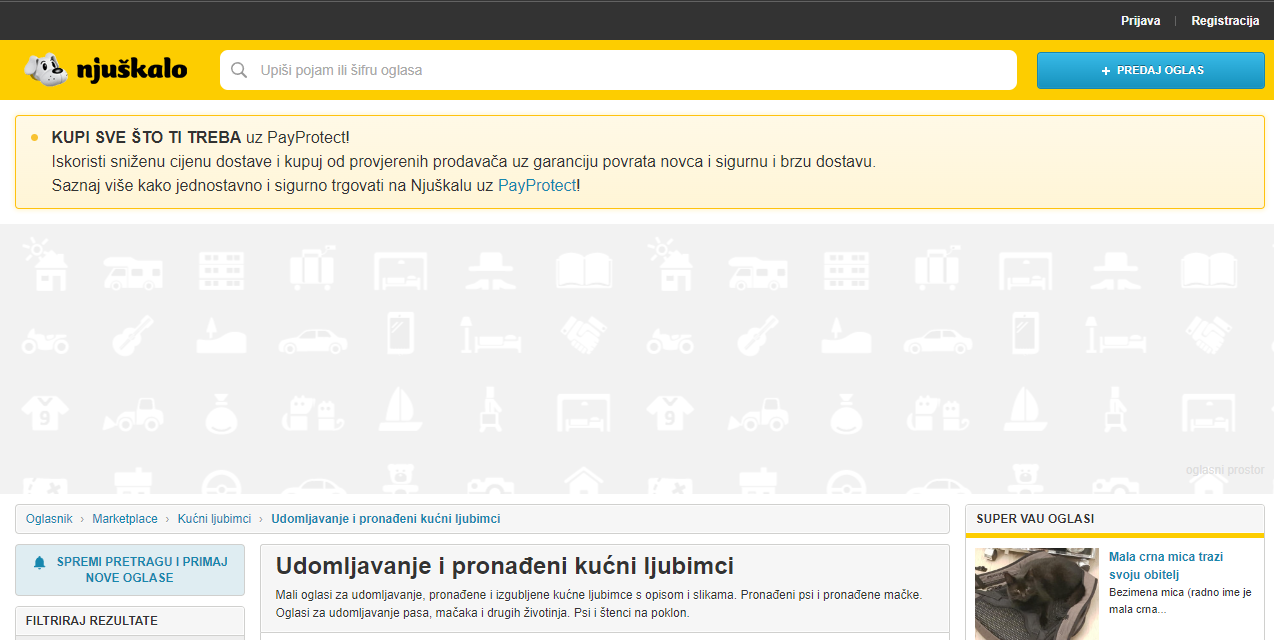
\includegraphics[scale=0.3]{slike/Njuskalo-nestaliLjubimci.PNG}
			\caption{Njuškalo}
			\label{fig:promjene}
		\end{figure}
		
		\textit{Web aplikacija za pronalazak nestalih ljubimaca će predstavljati puno učinkovitije rješenje u kojem će se korisnici lako i brzo snalaziti. Dodatno, važno je istaknuti da će svaki oglas za izgubljenog ljubimca, zajedno s odgovarajućom komunikacijom, biti tretiran kao samostalna i odvojena cjelina, bez međusobnih preklapanja s drugim oglasima. Ovim pristupom će biti osigurana jednostavna i brza pretraga unutar objavljenih oglasa, što će rezultirati znatno poboljšanom učinkovitošću i brzinom u usporedbi s tradicionalnim platformama poput Facebooka ili Njuškala.}
		
		\textit{Prilagodbe rješenja i nadogradnje projektnog zadatka bit će moguće u budućnosti, uz naglasak na korisničkom zadovoljstvu i njihovim mišljenjima. Korisnike se potiče da iznose svoja moguća rješenja i sugestije kako bi se unaprijedila web aplikacija te postala sve korisnija, učinkovitija i uspješnija u pomoći korisnicima u potrazi za izgubljenim ljubimcima.}
		
		\eject
		
		
	
	\chapter{Specifikacija programske potpore}
		
	\section{Funkcionalni zahtjevi}
			
			\textbf{\textit{dio 1. revizije}}\\
			
			\textit{Navesti \textbf{dionike} koji imaju \textbf{interes u ovom sustavu} ili  \textbf{su nositelji odgovornosti}. To su prije svega korisnici, ali i administratori sustava, naručitelji, razvojni tim.}\\
				
			\textit{Navesti \textbf{aktore} koji izravno \textbf{koriste} ili \textbf{komuniciraju sa sustavom}. Oni mogu imati inicijatorsku ulogu, tj. započinju određene procese u sustavu ili samo sudioničku ulogu, tj. obavljaju određeni posao. Za svakog aktora navesti funkcionalne zahtjeve koji se na njega odnose.}\\
			
			
			\noindent \textbf{Dionici:}
			
			\begin{packed_enum}
				
				\item Dionik 1
				\item Dionik 2				
				\item ...
				
			\end{packed_enum}
			
			\noindent \textbf{Aktori i njihovi funkcionalni zahtjevi:}
			
			
			\begin{packed_enum}
				\item  \underbar{Aktor 1 (inicijator) može:}
				
				\begin{packed_enum}
					
					\item funkcionalnost 1
					\item funkcionalnost 2
					\begin{packed_enum}
						
						\item  podfunkcionalnost 1 
						\item  podfunkcionalnost 2
				
					\end{packed_enum}
					\item  funkcionalnost 3
					
				\end{packed_enum}
			
				\item  \underbar{Aktor 2 (sudionik) može:}
				
				\begin{packed_enum}
					
					\item funkcionalnost 1
					\item funkcionalnost 2
					
				\end{packed_enum}
			\end{packed_enum}
			
			\eject 
			
			
				
			\subsection{Obrasci uporabe}
				
				\textbf{\textit{dio 1. revizije}}
				
				\subsubsection{Opis obrazaca uporabe}		

					\noindent \underbar{\textbf{UC1 - Pregled nestalih ljubimaca}}
					\begin{packed_item}
	
						\item \textbf{Glavni sudionik: }Korisnik, Registrirani korisnik, Sklonište
						\item  \textbf{Cilj:} Pregledavanje oglašenih nestalih kućnih ljubimaca i skloništa za životinje
						\item  \textbf{Sudionici:} Baza podataka
						\item  \textbf{Preduvjet:} -
						\item  \textbf{Opis osnovnog tijeka:}
						
						\item[] \begin{packed_enum}
	
							\item Nestali ljubimci su prikazani prilikom učitavanja aplikacije
							\item Korisnik odabire nestalog ljubimca
							\item Prikazuje se detaljniji pregled informacija i pregled komunikacija oko potrage
						\end{packed_enum}
						
					\end{packed_item}
				
					\noindent \underbar{\textbf{UC2 - Registracija}}
					\begin{packed_item}
						
						\item \textbf{Glavni sudionik: }Korisnik 
						\item  \textbf{Cilj:} Stvoriti korisnički račun za pristup sustavu
						\item  \textbf{Sudionici:} Baza podataka
						\item  \textbf{Preduvjet:} -
						\item  \textbf{Opis osnovnog tijeka:}
						
						\item[] \begin{packed_enum}
							
							\item Korisnik odabire opciju za registraciju
							\item Korisnik unosi vlastite podatke
							\item Podaci se spremaju u bazu podataka
							\item Korisnik prima obavijest o uspješnoj registraciji
						\end{packed_enum}
						
						\item  \textbf{Opis mogućih odstupanja:}
						
						\item[] \begin{packed_item}
							
							\item[2.a] Podaci koje je korisnik unio odgovaraju postojećem korisničkom računu
							\item[] \begin{packed_enum}
								
								\item Pojavljuje se poruka o neuspješnoj registraciji i zahtjev za ponovnim unosom podataka
								\item Korisnik mijenja podatke ili odustaje od registracije
								
							\end{packed_enum}
							\item[2.b] Korisnik nije unio sve zahtijevane podatke
								\item[] \begin{packed_enum}
								
								\item Pojavljuje se poruka o neuspješnoj registraciji i zahtjev za ponovnim unosom podataka
								\item Korisnik unosi zahtijevane podatke ili odustaje od registracije
								
							\end{packed_enum}
							
						\end{packed_item}
					\end{packed_item}
					
					\noindent \underbar{\textbf{UC3 - Pretraživanje nestalih ljubimaca}}
					\begin{packed_item}
						
						\item \textbf{Glavni sudionik: }Korisnik, Registrirani korisnik, Sklonište
						\item  \textbf{Cilj:} Pretraživanje nestalih ljubimaca po svim dostupnim kategorijama podataka
						\item  \textbf{Sudionici:} Baza podataka
						\item  \textbf{Preduvjet:} -
						\item  \textbf{Opis osnovnog tijeka:}
						
						\item[] \begin{packed_enum}
							
							\item Korisnik odabire kategorije podataka po kojima obavlja pretraživanje
							\item Korisnik unosi podatke (filtre) za odabrane kategorije
							\item Prikazuje se popis filtriranih oglasa
						\end{packed_enum}
					\end{packed_item}
					
					\noindent \underbar{\textbf{UC4 - Prijava u sustav}}
					\begin{packed_item}
						
						\item \textbf{Glavni sudionik: }Registrirani korisnik, Sklonište
						\item  \textbf{Cilj:} Dobiti pristup korisničkom sučelju
						\item  \textbf{Sudionici:} Baza podataka
						\item  \textbf{Preduvjet:} Registracija
						\item  \textbf{Opis osnovnog tijeka:}
						
						\item[] \begin{packed_enum}
							
							\item Unos korisničkog imena ili e-mail adrese i lozinke
							\item Provjera ispravnosti unesenih podataka
							\item Pristup korisničkom sučelju web aplikacije
						\end{packed_enum}
						
						\item  \textbf{Opis mogućih odstupanja:}
						
						\item[] \begin{packed_item}
							
							\item[2.a] Korisnik je unio nepostojeće korisničko ime ili e-mail adresu
							\item[] \begin{packed_enum}
								
								\item Pojavljuje se poruka o neuspješnoj prijavi i zahtjev za ponovnim unosom podataka
								\item Korisnik unosi ispravne podatke ili odustaje od prijave
								
							\end{packed_enum}
							\item[2.b] Korisnik je unio neispravnu lozinku za odgovarajuće korisničko ime odnosno e-mail
							\item[] \begin{packed_enum}
								
								\item Pojavljuje se poruka o neuspješnoj prijavi i zahtjev za ponovnim unosom podataka
								\item Korisnik unosi ispravne podatke ili odustaje od prijave
								
							\end{packed_enum}
							
						\end{packed_item}
					\end{packed_item}
					\pagebreak
					\noindent \underbar{\textbf{UC5 - Komuniciranje oko potrage}}
					\begin{packed_item}
						
						\item \textbf{Glavni sudionik: }Registrirani korisnik, Sklonište
						\item  \textbf{Cilj:} Ostvariti komunikaciju s vlasnikom izgubljenog ljubimca
						\item  \textbf{Sudionici:} Baza podataka
						\item  \textbf{Preduvjet:} Korisnik je prijavljen
						\item  \textbf{Opis osnovnog tijeka:}
						
						\item[] \begin{packed_enum}
							
							\item Korisnik odabire nestalog ljubimca
							\item Prikazuje se popis komunikacije oko potrage za ljubimcem
							\item Korisnik unosi poruku koja može sadržavati tekst, sliku i geolokaciju
						\end{packed_enum}
					\end{packed_item}
					
					\noindent \underbar{\textbf{UC6.1 - Postavljanje oglasa}}
					\begin{packed_item}
						
						\item \textbf{Glavni sudionik: }Registrirani korisnik, Sklonište 
						\item  \textbf{Cilj:} Postaviti oglas o izgubljenom ljubimcu
						\item  \textbf{Sudionici:} Baza podataka
						\item  \textbf{Preduvjet:} Korisnik je prijavljen
						\item  \textbf{Opis osnovnog tijeka:}
						
						\item[] \begin{packed_enum}
							
							\item Korisnik odabire opciju za novi oglas
							\item Korisnik unosi podatke o ljubimcu za zadane kategorije
							\item Korisnik objavljuje oglas
						\end{packed_enum}
						
						\item  \textbf{Opis mogućih odstupanja:}
						
						\item[] \begin{packed_item}
							
							\item[2.a] Korisnik je unio invalidne podatke u određenu kategoriju
							\item[] \begin{packed_enum}
								
								\item Pojavljuje se poruka o pogrešci i zahtjev za ponovnim unosom podataka
								\item Korisnik unosi ispravne podatke ili odustaje od objave oglasa
								
							\end{packed_enum}
							\item[2.b] Korisnik nije unio potrebne podatke
							\item[] \begin{packed_enum}
								
								\item Pojavljuje se poruka o pogrešci i zahtjev za ponovnim unosom podataka
								\item Korisnik unosi zahtijevane podatke ili odustaje od objave oglasa
								
							\end{packed_enum}
						\end{packed_item}
					\end{packed_item}
					\pagebreak
					\noindent \underbar{\textbf{UC6.2 - Uklanjanje oglasa}}
					\begin{packed_item}
						
						\item \textbf{Glavni sudionik: }Registrirani korisnik, Sklonište
						\item  \textbf{Cilj:} Ukloniti oglas o izgubljenom ljubimcu
						\item  \textbf{Sudionici:} Baza podataka
						\item  \textbf{Preduvjet:} Korisnik je prijavljen i objavio je oglas
						\item  \textbf{Opis osnovnog tijeka:}
						
						\item[] \begin{packed_enum}
							
							\item Korisnik odabire opciju za brisanje oglasa
							\item Korisnik potvrđuje akciju brisanja
							\item Oglas i sva komunikacija vezana uz njega nestaju iz popisa vidljivih oglasa
							\item Oglas ostaje pohranjen u bazi podataka
						\end{packed_enum}
						
						\item  \textbf{Opis mogućih odstupanja:}
						
						\item[] \begin{packed_item}
							
							\item[2.a] Korisnik odustaje od brisanja oglasa
						\end{packed_item}
					\end{packed_item}
					
					\noindent \underbar{\textbf{UC6.3 - Izmjena oglasa}}
					\begin{packed_item}
						
						\item \textbf{Glavni sudionik: }Registrirani korisnik, Sklonište
						\item  \textbf{Cilj:} Izmjena oglasa o izgubljenom ljubimcu
						\item  \textbf{Sudionici:} Baza podataka
						\item  \textbf{Preduvjet:} Korisnik je prijavljen i objavio je oglas
						\item  \textbf{Opis osnovnog tijeka:}
						
						\item[] \begin{packed_enum}
							
							\item Korisnik odabire opciju za izmjenu oglasa
							\item 
								\begin{packed_item}
									\item[a$)$] Korisnik mijenja podatke po kategorijama oglasa
									\item[b$)$] Korisnik mijenja kategoriju oglasa 
								\end{packed_item}
							\item Korisnik sprema promjene
						\end{packed_enum}
						
						\item  \textbf{Opis mogućih odstupanja:}
						
						\item[] \begin{packed_item}
							
							\item[2.a] Korisnik je unio invalidne podatke u određenu kategoriju
							\item[] \begin{packed_enum}
								
								\item  Pojavljuje se poruka o pogrešci i zahtjev za ponovnim unosom
								\item Korisnik unosi ispravne podatke ili odustaje od izmjene oglasa
								
							\end{packed_enum}
							\item[2.b] Korisnik je promijenio kategoriju oglasa u kategoriju koja ne odgovara aktivnoj potrazi za ljubimcem
							\begin{packed_enum}
								
								\item Oglas se prebacuje u popis neaktivnih oglasa
								
							\end{packed_enum}
							
						\end{packed_item}
					\end{packed_item}
					\pagebreak
					\noindent \underbar{\textbf{UC7 - Oglašavanje pronađenih životinja}}
					\begin{packed_item}
						
						\item \textbf{Glavni sudionik: }Sklonište
						\item  \textbf{Cilj:} Oglašavanje pronađenih životinja koje se nalaze u prostoru skloništa
						\item  \textbf{Sudionici:} Baza podataka
						\item  \textbf{Preduvjet:} Korisnik je prijavljen
						\item  \textbf{Opis osnovnog tijeka:}
						
						\item[] \begin{packed_enum}
							
							\item Korisnik odabire opciju za novi oglas
							\item Korisnik unosi podatke o ljubimcu za zadane kategorije (uključujući i dodatnu kategoriju – u skloništu)
							\item Korisnik objavljuje oglas
						\end{packed_enum}
						
						\item  \textbf{Opis mogućih odstupanja:}
						
						\item[] \begin{packed_item}
							
							\item[2.a] Korisnik je unio invalidne podatke u određenu kategoriju
							\item[] \begin{packed_enum}
								
								\item Pojavljuje se poruka o pogrešci i zahtjev za ponovnim unosom podataka
								\item Korisnik unosi ispravne podatke ili odustaje od objave oglasa
								
							\end{packed_enum}
							\item[2.b] Korisnik nije unio potrebne podatke
							\item[] \begin{packed_enum}
								
								\item Pojavljuje se poruka o pogrešci i zahtjev za ponovnim unosom podataka
								\item Korisnik unosi zahtijevane podatke ili odustaje od objave oglasa
								
							\end{packed_enum}
						\end{packed_item}
					\end{packed_item}
					
				
					
				\pagebreak
				\subsubsection{Dijagrami obrazaca uporabe}
				
					\begin{figure}[htb]
						\centering
						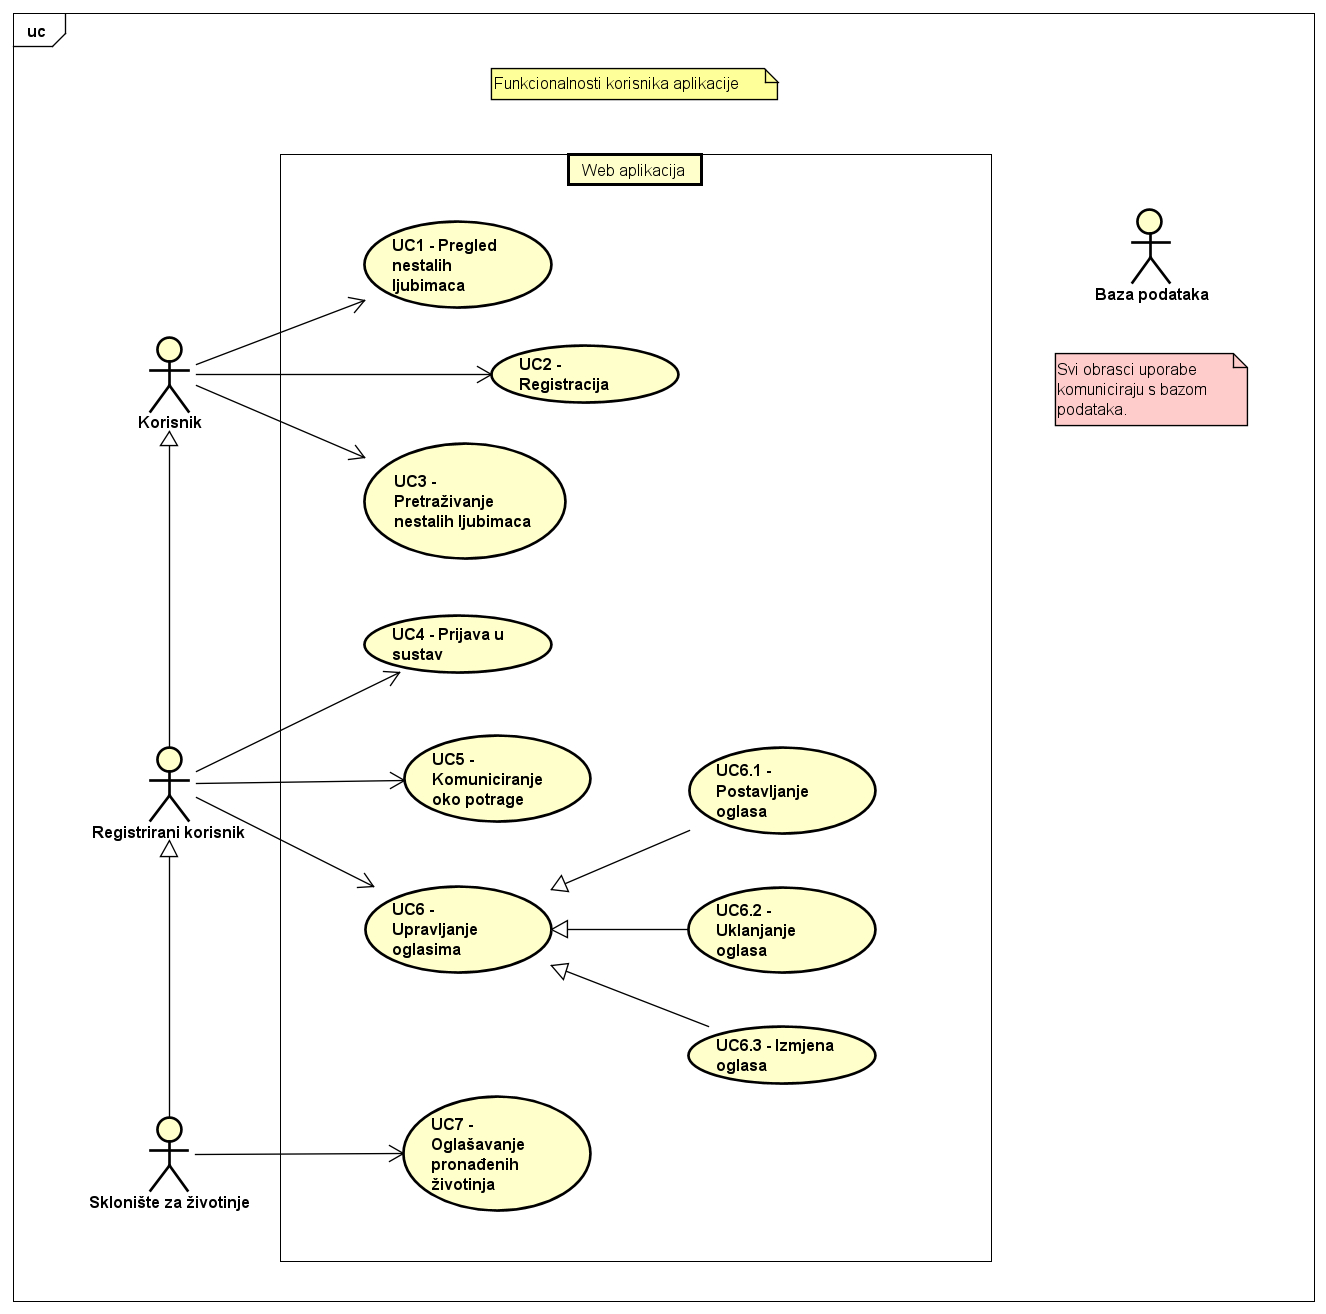
\includegraphics[width=\textwidth]{slike/funkcionalnosti_korisnika.png}
						\caption{Dijagram obrasca uporabe, funkcionalnost korisnika}
					\end{figure}		
				
			\pagebreak
			\subsection{Sekvencijski dijagrami}
				
				\textbf{\textit{dio 1. revizije}}\\
				
				\textit{Nacrtati sekvencijske dijagrame koji modeliraju najvažnije dijelove sustava (max. 4 dijagrama). Ukoliko postoji nedoumica oko odabira, razjasniti s asistentom. Uz svaki dijagram napisati detaljni opis dijagrama.}
				\eject
	
		\section{Ostali zahtjevi}
		
			\textbf{\textit{dio 1. revizije}}\\
		 
			 \textit{Nefunkcionalni zahtjevi i zahtjevi domene primjene dopunjuju funkcionalne zahtjeve. Oni opisuju \textbf{kako se sustav treba ponašati} i koja \textbf{ograničenja} treba poštivati (performanse, korisničko iskustvo, pouzdanost, standardi kvalitete, sigurnost...). Primjeri takvih zahtjeva u Vašem projektu mogu biti: podržani jezici korisničkog sučelja, vrijeme odziva, najveći mogući podržani broj korisnika, podržane web/mobilne platforme, razina zaštite (protokoli komunikacije, kriptiranje...)... Svaki takav zahtjev potrebno je navesti u jednoj ili dvije rečenice.}
			 
			 
			 
	
	\chapter{Arhitektura i dizajn sustava}
		
		\textbf{\textit{dio 1. revizije}}\\

		Arhitektura koju koristimo se zasniva na MVC (Model-View-Controller) konceptu, varijacije arhitekture zasnovane na događajima.
        \\
        \\
        Cjelokupni sustav se može podijeliti na četiri glavne komponente:
            \begin{itemize}
                \item Web preglednik
                \item Web poslužitelj (server)
                \item Web aplikaciju
                \item Bazu podataka
            \end{itemize}
    
        \begin{figure}[h]
            \centering
            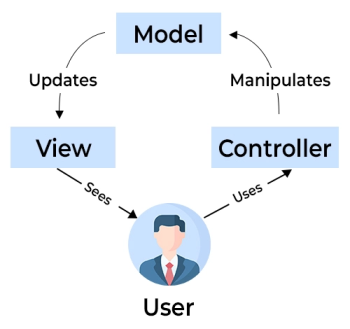
\includegraphics[width=0.5\textwidth]{slike/mvc.png}
            \caption{MVC model}
            \label{fig:mesh1}
        \end{figure}
        
        \textbf{Web preglednik} je program (software) koji omogućava korisnicima pregledavanje i prikazivanje web stranica na World Wide Webu (WWW). Predstavlja sučelje između korisnika i internetskog sadržaja. Pomoću njega korisnik sustava komunicira s web aplikacijom, točnije \textit{View} i \textit{Controller} komponentom.
        
        \pagebreak

        \textbf{Web aplikaciju} pokreće \textbf{poslužitelj}. To je program čiji je osnovni zadatak odgovarati na HTTP (\textit{Hyper Text Transfer Protocol}) zahtjeve klijenata, primati i slati određene resurse - posluživati samu aplikaciju. 
        
        \begingroup 
        U većini slučajeva klijent će zahtjevati pristup podacima kojima web poslužitelj nema pristup. U tom slučaju će \textit{Controller} komponenta poslati zahtjev \textit{Model} komponenti, zaslužnoj za pohranu korisničkih podataka, koju u našem slučaju predstavlja \textbf{baza podataka}. 
        \endgroup
        
        \begingroup
        Baza podataka organizirana je zbirka logički povezanih, pretražljivih i međusobno ovisnih podataka. Ključna je komponenta mnogih aplikacija i sustava zbog mogućnosti sigurne pohrane i brzog pretraživanja SQL upitima.
	  \endgroup

        \begingroup
        Za našu implementaciju korisničkog sučelja odabrali smo programski jezik \textit{JavaScript} s bibliotekom \textit{React}. Za implementaciju poslužiteljske strane odabrali smo programski jezik \textit{Java} i \textit{Spring} framework, točnije proširenje \textit{Spring Boot}. Kao razvojnu okolinu odabrali smo \textit{Visual Studio Code} i \textit{JetBrains IntelliJ IDEA}. Za implementaciju baze podataka odabrali smo \textit{PostgreSQL}.
        \endgroup

		\begin{figure}[h]
            \centering
            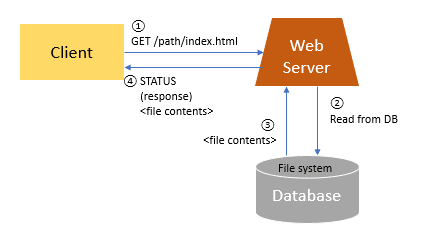
\includegraphics[width=1\textwidth]{slike/client-server-db.png}
            \caption{Prikaz osnovnog rada sustava}
            \label{fig:mesh1}
        \end{figure}

        \pagebreak
				
		\section{Baza podataka}
			
			\textbf{\textit{dio 1. revizije}}\\
			
		\textit{Potrebno je opisati koju vrstu i implementaciju baze podataka ste odabrali, glavne komponente od kojih se sastoji i slično.}
		
			\subsection{Opis tablica}
			

				\textit{Svaku tablicu je potrebno opisati po zadanom predlošku. Lijevo se nalazi točno ime varijable u bazi podataka, u sredini se nalazi tip podataka, a desno se nalazi opis varijable. Svjetlozelenom bojom označite primarni ključ. Svjetlo plavom označite strani ključ}
				
				
				\begin{longtblr}[
					label=none,
					entry=none
					]{
						width = \textwidth,
						colspec={|X[6,l]|X[6, l]|X[20, l]|}, 
						rowhead = 1,
					} %definicija širine tablice, širine stupaca, poravnanje i broja redaka naslova tablice
					\hline \SetCell[c=3]{c}{\textbf{korisnik - ime tablice}}	 \\ \hline[3pt]
					\SetCell{LightGreen}IDKorisnik & INT	&  	Lorem ipsum dolor sit amet, consectetur adipiscing elit, sed do eiusmod  	\\ \hline
					korisnickoIme	& VARCHAR &   	\\ \hline 
					email & VARCHAR &   \\ \hline 
					ime & VARCHAR	&  		\\ \hline 
					\SetCell{LightBlue} primjer	& VARCHAR &   	\\ \hline 
				\end{longtblr}
				
				
			
			\subsection{Dijagram baze podataka}
				\textit{ U ovom potpoglavlju potrebno je umetnuti dijagram baze podataka. Primarni i strani ključevi moraju biti označeni, a tablice povezane. Bazu podataka je potrebno normalizirati. Podsjetite se kolegija "Baze podataka".}
			
			\eject
			
			
		\section{Dijagram razreda}
		
			\textit{Potrebno je priložiti dijagram razreda s pripadajućim opisom. Zbog preglednosti je moguće dijagram razlomiti na više njih, ali moraju biti grupirani prema sličnim razinama apstrakcije i srodnim funkcionalnostima.}\\
			
			\textbf{\textit{dio 1. revizije}}\\
			
			\textit{Prilikom prve predaje projekta, potrebno je priložiti potpuno razrađen dijagram razreda vezan uz \textbf{generičku funkcionalnost} sustava. Ostale funkcionalnosti trebaju biti idejno razrađene u dijagramu sa sljedećim komponentama: nazivi razreda, nazivi metoda i vrste pristupa metodama (npr. javni, zaštićeni), nazivi atributa razreda, veze i odnosi između razreda.}\\
			
			\textbf{\textit{dio 2. revizije}}\\			
			
			\textit{Prilikom druge predaje projekta dijagram razreda i opisi moraju odgovarati stvarnom stanju implementacije}
			
			
			
			\eject
		
		\section{Dijagram stanja}
			
			
			\textbf{\textit{dio 2. revizije}}\\
			
			\textit{Potrebno je priložiti dijagram stanja i opisati ga. Dovoljan je jedan dijagram stanja koji prikazuje \textbf{značajan dio funkcionalnosti} sustava. Na primjer, stanja korisničkog sučelja i tijek korištenja neke ključne funkcionalnosti jesu značajan dio sustava, a registracija i prijava nisu. }
			
			
			\eject 
		
		\section{Dijagram aktivnosti}
			
			\textbf{\textit{dio 2. revizije}}\\
			
			 \textit{Potrebno je priložiti dijagram aktivnosti s pripadajućim opisom. Dijagram aktivnosti treba prikazivati značajan dio sustava.}
			
			\eject
		\section{Dijagram komponenti}
		
			\textbf{\textit{dio 2. revizije}}\\
		
			 \textit{Potrebno je priložiti dijagram komponenti s pripadajućim opisom. Dijagram komponenti treba prikazivati strukturu cijele aplikacije.}
	\chapter{Implementacija i korisničko sučelje}


\section{Korištene tehnologije i alati}

Komunikacija u timu realizirana je korištenjem aplikacije \underline{Discord}\footnote{https://discord.com/}. Za izradu UML dijagrama korišten je alat \underline{Astah Professional}\footnote{https://astah.net/products/astah-professional/}, a kao sustav za upravljanje izvornim kodom \underline{Git}\footnote{https://git-scm.com/}. Udaljeni repozitorij projekta je dostupan na web platformi \underline{GitHub}\footnote{https://github.com/}.

Kao razvojno okruženje korišten je \underline{IntelliJ IDEA}\footnote{https://www.jetbrains.com/idea/} - integrirano je razvojno \newline okruženje (IDE) tvrtke JetBrains. Prvenstveno se koristi za razvoj računalnih programa za operacijski sustav Windows, kao i za web-stranice, web-aplikacije, web-usluge i mobilne aplikacije. IntelliJ IDEA za razvoj softvera koristi JetBrains platforme i tehnologije za olakšavanje procesa razvoja. To uključuje podršku za razvoj u raznim programskim jezicima(poput Java, Kotlin, Groovy i mnogih drugih), za Android razvoj, Spring Framework, Web development(\textit{frontend} i \textit{backend}) itd. Uz IntelliJ IDEA ponešto je korišten i \underline{Visual Studio Code}\footnote{https://code.visualstudio.com/}, ali uglavnom kao text editor te za pisanje \underline{docker}\footnote{https://www.docker.com/} deploy skripte. Docker predstavlja platformu kao uslugu(Paas) koja koristi virtualizaciju na razini OS-a za isporuku programa u spremnicima. Spremnici osiguravaju izolaciju procesa, mreže i datotečnog sustava.

Aplikacija je napisana koristeći radni okvir \underline{Spring Framework}\footnote{https://spring.io/} i jezik \underline{Java}\footnote{https://www.java.com/en/} za izradu \textit{backenda} te \underline{React}\footnote{https://react.dev/} i jezik \underline{TypeScript}\footnote{https://www.typescriptlang.org/} za izradu \textit{frontenda}. React, također poznat kao React.js ili ReactJS, je biblioteka u JavaScriptu za izgradnju korisničkih sučelja. Održavana je od strane Facebooka. React se najčešće koristi kao osnova u razvoju web ili mobilnih aplikacija. Složene aplikacije u Reactu obično zahtijevaju korištenje dodatnih biblioteka za interakciju s API-jem. Programski jezik TypeScript je nadogradnja na JavaScript, a napravio ga je Microsoft. Radni okvir Spring Framework nadograđuje mogućnosti samog operativnog sustava. Radi se o posebnoj infrastrukturi koja programerima nudi gotova rješenja i funkcionalnosti da bi ubrzala i pojednostavila razvoj aplikacija svih vrsta i oblika.

Baza podataka se nalazi na poslužitelju u oblaku \underline{Render}\footnote{https://render.com/}.

\eject


\section{Ispitivanje programskog rješenja}

\subsection{Ispitivanje komponenti}
Ispitivanje komponenti sustava smo proveli uz pomoć alata \underline{JUnit} \footnote{https://junit.org/junit5/}, okvira za jedinično testiranje za programski jezik Java koji je iznimno važan u razvoju vođenom testiranjem. Pri razvoju aplikacije korištena je inačica 5.

\text{Izvorni kôd svih ispitnih slučajeva i rezultati izvođenja ispita prikazani su u nastavku}
\renewcommand{\lstlistingname}{Kod}
\begin{lstlisting}[
	language=Java,
	frame=single,
	label={lst:testGetAllRequestedAdvertisements},
	basicstyle = \small,
	tabsize=2,
	showspaces=false,
	showstringspaces=false,
	commentstyle = \color{red}, %% set comment color
	keywordstyle = \color{blue}, %% set keyword color
	stringstyle = \color{applegreen}, %% set string color
	rulecolor = \color{black},
	caption={Test testGetAllRequestedAdvertisements},
	breaklines=true]
	@Test
	@DisplayName("All requested advertisements are fetched")
	public void testGetAllRequestedAdvertisements() {
		
		Advertisement advertisement1 = mock(Advertisement.class);
		when(advertisement1.getAdState()).thenReturn(AdStateEnum.ACTIVE);
		when(advertisement1.getCategory()).thenReturn(CategoryEnum.LJUBIMAC_JE_SRETNO_PRONADEN);
		
		Advertisement advertisement2 = mock(Advertisement.class);
		when(advertisement2.getAdState()).thenReturn(AdStateEnum.ACTIVE);
		when(advertisement2.getCategory()).thenReturn(CategoryEnum.LJUBIMAC_JE_NESTAO_I_ZA_NJIM_SE_TRAGA);
		when(advertisement2.getPet()).thenReturn(mock(Pet.class));
		when(advertisement2.getUser()).thenReturn(mock(Registered.class));
		when(imageRepository.findAllByPetPetId(anyLong())).thenReturn(Arrays.asList(mock(Image.class)));
		
		when(advertisementRepository.findAll()).thenReturn(Arrays.asList(
		advertisement1, advertisement2)
		);
		
		List<AdvertisementSummaryDTO> result = advertisementService.getAllAdvertisements(
		CategoryEnum.LJUBIMAC_JE_NESTAO_I_ZA_NJIM_SE_TRAGA
		);
		
		assertEquals(1, result.size());
	}
\end{lstlisting}

U Kodu \ref{lst:testGetAllRequestedAdvertisements} prikazuje se ispitni slučaj koji osigurava da metoda AdvertisementService.getAllAdvertisements(CategoryEnum category) ispravno dohvaća i vraća oglase koji odgovaraju zadanom kriteriju kategorije. Kreiraju se dva mock (simulirana) oglasa (advertisement1 i advertisement2) koristeći Mockito okvir za testiranje. Oba oglasa su postavljena na aktivno stanje (AdStateEnum.ACTIVE), ali pripadaju različitim kategorijama. S obzirom da samo 1 objekt pripada traženoj kategoriji (advertisement2), sa assertEquals(1, result.size()) provjeravamo jesmo li dobili samo 1 oglas.

\pagebreak

\begin{lstlisting}[
	language=Java,
	frame=single,
	label={lst:testNoneAdsOfRequestedCategoryFound},
	basicstyle = \small,
	tabsize=2,
	showspaces=false,
	showstringspaces=false,
	commentstyle = \color{red}, %% set comment color
	keywordstyle = \color{blue}, %% set keyword color
	stringstyle = \color{applegreen}, %% set string color
	rulecolor = \color{black},
	caption={Test testNoneAdsOfRequestedCategoryFound},
	breaklines=true]
	@Test
	@DisplayName("Having zero advertisements of requested category is handled correctly")
	public void testNoneAdsOfRequestedCategoryFound() {
		
		Advertisement advertisement1 = mock(Advertisement.class);
		when(advertisement1.getAdState()).thenReturn(AdStateEnum.DELETED);
		
		Advertisement advertisement2 = mock(Advertisement.class);
		when(advertisement2.getAdState()).thenReturn(AdStateEnum.ACTIVE);
		when(advertisement2.getCategory()).thenReturn(CategoryEnum.LJUBIMAC_JE_SRETNO_PRONADEN);
		
		when(advertisementRepository.findAll()).thenReturn(Arrays.asList(
		advertisement1, advertisement2)
		);
		
		List<AdvertisementSummaryDTO> result = advertisementService.getAllAdvertisements(
		CategoryEnum.LJUBIMAC_JE_PRONADEN_U_NESRETNIM_OKOLNOSTIMA
		);
		
		assertEquals(0, result.size());
	}
\end{lstlisting}

U Kodu \ref{lst:testNoneAdsOfRequestedCategoryFound} prikazuje se ispitni slučaj koji, kao i u prethodnom ispitnom slučaju, ispituje funkcionalnost metode  AdvertisementService.getAllAdvertisements(CategoryEnum category), ali ovaj put ispitujemo rubni slučaj: u bazi ne postoji oglas koji ispunjava korisnički zadane kriterije (ili ne pripada traženoj kategoriji ili je "obrisan"). Sa assertEquals(0, result.size()) provjeravamo je li povratna vrijednost metode ispitivane metode prazna lista. 

\pagebreak

\begin{lstlisting}[
	language=Java,
	frame=single,
	label={lst:testRegisteredUserCannotSetInShelterCategory},
	basicstyle = \small,
	tabsize=2,
	showspaces=false,
	showstringspaces=false,
	commentstyle = \color{red}, %% set comment color
	keywordstyle = \color{blue}, %% set keyword color
	stringstyle = \color{applegreen}, %% set string color
	rulecolor = \color{black},
	caption={Test testRegisteredUserCannotSetInShelterCategory},
	breaklines=true]
	@Test
	@DisplayName("Non-shelter user cannot set U_SKLONISTU category")
	public void testRegisteredUserCannotSetInShelterCategory() {
		
		assertThrows(SecurityException.class, () -> {
			
			Long adId = 1L;
			AddAdvertisementDTO dto = mock(AddAdvertisementDTO.class);
			when(dto.getCategory()).thenReturn(CategoryEnum.U_SKLONISTU);
			when(dto.getDisappearanceLocationLat()).thenReturn(null);
			
			when(advertisementRepository.existsByAdvertisementId(anyLong())).thenReturn(true);
			
			Advertisement changedAdvertisement = mock(Advertisement.class);
			when(changedAdvertisement.getUser()).thenReturn(mock(Registered.class));
			
			when(advertisementRepository.findByAdvertisementId(anyLong())).thenReturn(Optional.of(changedAdvertisement));
			
			advertisementService.changeAdvertisement(adId, dto);
		});
	}
\end{lstlisting}

U Kodu \ref{lst:testRegisteredUserCannotSetInShelterCategory} nalazi se ispitni slučaj koji provjerava ispravnost rada metode AdvertisementService.changeAdvertisement(long adId, AddAdvertisementDTO dto). Testira se slučaj kada obični (registrirani) korisnik pokušava promijeniti svoj oglas tako da mu postavi kategoriju "U SKLONISTU". S obzirom da on nema dopuštenje za postavljanje te kategorije (nije sklonište), metoda changeAdvertisement() bi trebala baciti SecurityException iznimku, što i provjeravamo sa kodnim isječkom assertThrows(SecurityException.class, ...).

\pagebreak

\begin{figure}[!htb]
	\centering
	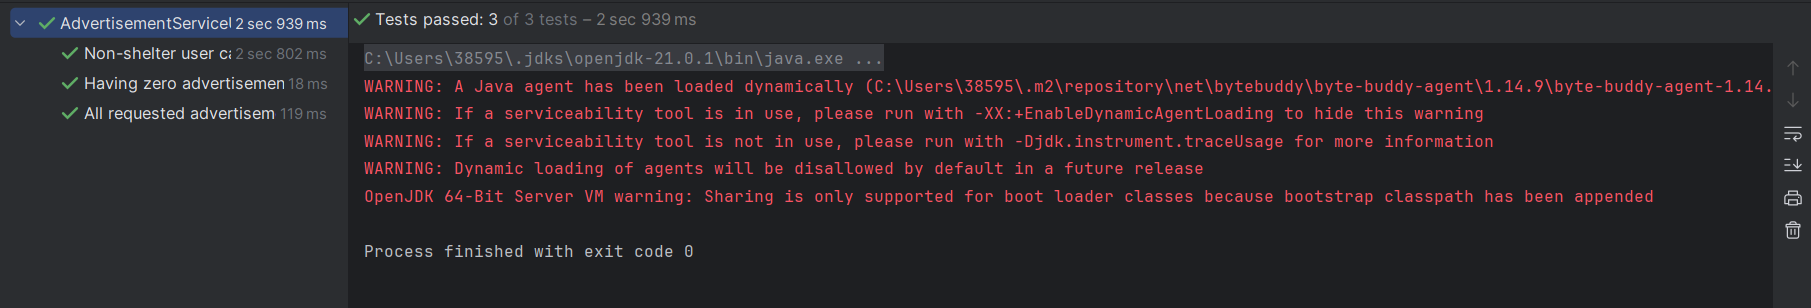
\includegraphics[width=\textwidth]{slike/test1.png}
	\caption{Testovi prolaze}
\end{figure}

\begin{lstlisting}[
	language=Java,
	frame=single,
	label={lst:testGetLocation},
	basicstyle = \small,
	tabsize=2,
	showspaces=false,
	showstringspaces=false,
	commentstyle = \color{red}, %% set comment color
	keywordstyle = \color{blue}, %% set keyword color
	stringstyle = \color{applegreen}, %% set string color
	rulecolor = \color{black},
	caption={Test testGetLocation},
	breaklines=true]
	@BeforeEach
	public void setup() {
		locationService = new LocationService(countyRepository, placeRepository, locationRepository) {
			@Override
			protected MapsSummaryDTO getLocInfoFromAPI(double latitude, double longitude) {
				MapsSummaryDTO dto = new MapsSummaryDTO();
				dto.setLocationName("Zagreb");
				dto.setPlace("Zagreb");
				dto.setCounty("Grad Zagreb");
				dto.setPostalCode("10000");
				return dto;
			}
		};
	}
	
	@Test
	@DisplayName("Location objects are retrieved successfully")
	public void testGetLocation() {
		when(countyRepository.existsByName(anyString())).thenReturn(true);
		when(countyRepository.findByName(anyString())).thenReturn(Optional.of(new County("Grad Zagreb")));
		when(placeRepository.existsByZipCode(anyLong())).thenReturn(true);
		when(placeRepository.findByZipCode(anyLong())).thenReturn(Optional.of(
		new Place(10000L, "Zagreb", new County("Grad Zagreb"))
		));
		
		locationService.getLocation(45.815399, 15.966568);
		
		Mockito.verify(locationRepository, times(1)).save(any(Location.class));
		
	}
\end{lstlisting}

U Kodu \ref{lst:testRegisteredUserCannotSetInShelterCategory} osigurava da metoda LocationService.getLocation(double latitude, double longitude) ispravno dohvaća informacije o lokaciji s API-ja, pravilno interagira s repozitorijima i sprema dobivene informacije o lokaciji. Test provjerava je li metoda save() pozvana nad objektom locationRepository točno jednom: ako je, to znači da je implementacija metode ispravna prema ovom scenariju, a ako nije, to ukazuje na potencijalni problem u implementaciji metode. NAPOMENA: s obzirom da povezivanje na API pri izvođenju unit testa nije preporučeno, metoda getLocInfoFromAPI(double latitude, double longitude) je konfigurirana da uvijek vraća informacije o lokaciji Zagreb, bez obzira na ulazne parametre. 

\begin{figure}[!htb]
	\centering
	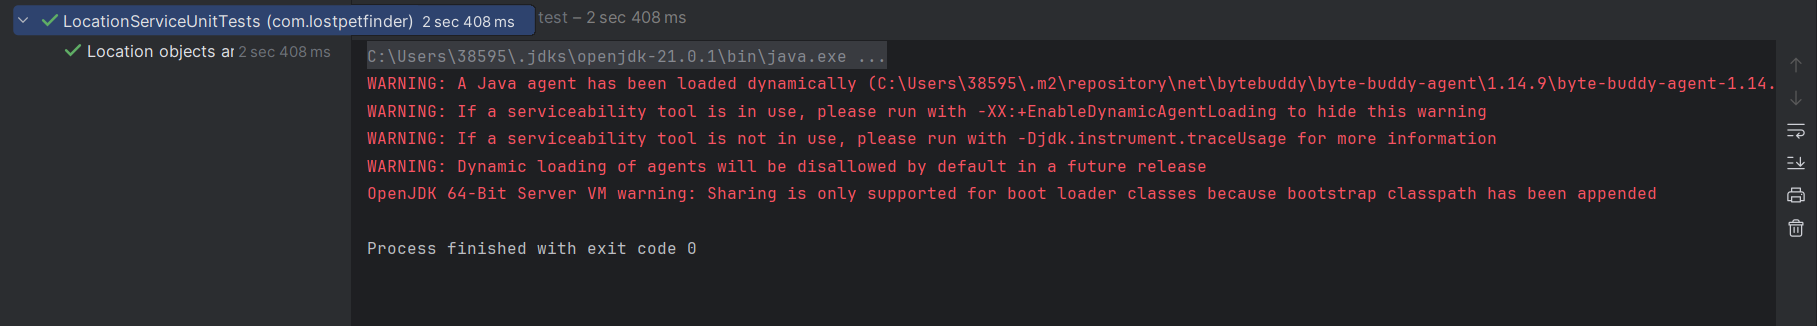
\includegraphics[width=\textwidth]{slike/test2.png}
	\caption{Test prolazi}
\end{figure}

\pagebreak

\begin{lstlisting}[
	language=Java,
	frame=single,
	label={lst:testSaveMessageWithTextOnly},
	basicstyle = \small,
	tabsize=2,
	showspaces=false,
	showstringspaces=false,
	commentstyle = \color{red}, %% set comment color
	keywordstyle = \color{blue}, %% set keyword color
	stringstyle = \color{applegreen}, %% set string color
	rulecolor = \color{black},
	caption={Test testSaveMessageWithTextOnly},
	breaklines=true]
	@Test
	@DisplayName("Messages with text only are successfully saved")
	public void testSaveMessageWithTextOnly() {
		
		MessageInputDTO dto = mock(MessageInputDTO.class);
		when(dto.getSenderUsername()).thenReturn("testUser");
		when(dto.getMessageText()).thenReturn("testMessageText");
		when(dto.getAdvertisementId()).thenReturn(1L);
		
		when(userRepository.findByUsername(anyString())).thenReturn(Optional.of(mock(User.class)));
		when(advertisementRepository.findByAdvertisementId(anyLong())).thenReturn(
		Optional.of(mock(Advertisement.class))
		);
		
		messageService.saveMessage(dto);
		
		Mockito.verify(messageRepository, times(1)).save(any(Message.class));
	}
\end{lstlisting}

U Kodu \ref{lst:testSaveMessageWithTextOnly} nalazi se ispitni slučaj koji  provjerava funkcionalnost metode MessageService.saveMessage(MessageInputDTO dto) kada je u sklopu poruke poslan tekst, ali ne i lokacija. Kreira se simulirani objekt MessageInputDTO pomoću metode mock() koji se zatim konfigurira da vrati “testUser” kao korisničko ime pošiljatelja, “testMessageText” kao tekst poruke i 1L kao ID oglasa. Metode findByUsername() u userRepository i findByAdvertisementId() u advertisementRepository su konfigurirane da uvijek vraćaju Optional objekt User i Advertisement, bez obzira na ulazne parametre. Metoda saveMessage se zatim poziva s prethodno kreiranim MessageInputDTO objektom. Na kraju, test provjerava je li metoda save() u messageRepository pozvana točno jednom.

\pagebreak

\begin{lstlisting}[
	language=Java,
	frame=single,
	label={lst:testSaveMessageWithLocationProvided},
	basicstyle = \small,
	tabsize=2,
	showspaces=false,
	showstringspaces=false,
	commentstyle = \color{red}, %% set comment color
	keywordstyle = \color{blue}, %% set keyword color
	stringstyle = \color{applegreen}, %% set string color
	rulecolor = \color{black},
	caption={Test testSaveMessageWithLocationProvided},
	breaklines=true]
	@Test
	@DisplayName("Messages with location included are successfully saved")
	public void testSaveMessageWithLocationProvided() {
		
		MessageInputDTO dto = mock(MessageInputDTO.class);
		when(dto.getSenderUsername()).thenReturn("testUser");
		when(dto.getMessageText()).thenReturn("testMessageText");
		when(dto.getAdvertisementId()).thenReturn(1L);
		when(dto.getDisappearanceLocationLat()).thenReturn(45.815399);
		when(dto.getDisappearanceLocationLng()).thenReturn(15.966568);
		
		when(userRepository.findByUsername(anyString())).thenReturn(Optional.of(mock(User.class)));
		when(advertisementRepository.findByAdvertisementId(anyLong())).thenReturn(
		Optional.of(mock(Advertisement.class))
		);
		when(locationRepository.existsByCoordinates(any(CoordinatesPK.class))).thenReturn(false);
		when(locationService.getLocation(anyDouble(), anyDouble())).thenReturn(mock(Location.class));
		
		messageService.saveMessage(dto);
		
		Mockito.verify(locationRepository, times(1)).save(any(Location.class));
		Mockito.verify(messageRepository, times(1)).save(any(Message.class));
	}
\end{lstlisting}

U Kodu \ref{lst:testSaveMessageWithLocationProvided} prikazuje se ispitni slučaj koji, kao i u prethodnom ispitnom slučaju, ispituje funkcionalnost metode MessageService.saveMessage(MessageInputDTO dto), ali u slučaju kada je lokacija zadana. Dio koda Mockito.verify(locationRepository, times(1)).save(any(Location.class)) provjerava je li pozvana metoda save() nad objektom locationRepository kako bi se utvrdilo da je zadana lokacija spremljena.

\pagebreak

\begin{lstlisting}[
	language=Java,
	frame=single,
	label={lst:testIfRetrievedChatMessagesAreOrdered},
	basicstyle = \small,
	tabsize=2,
	showspaces=false,
	showstringspaces=false,
	commentstyle = \color{red}, %% set comment color
	keywordstyle = \color{blue}, %% set keyword color
	stringstyle = \color{applegreen}, %% set string color
	rulecolor = \color{black},
	caption={Test testIfRetrievedChatMessagesAreOrdered},
	breaklines=true]
	@Test
	@DisplayName("Messages are retrieved in correct order")
	public void testIfRetrievedChatMessagesAreOrdered() {
		
		Message message1 = mock(Message.class);
		when(message1.getAltId()).thenReturn(new MessagePK(mock(User.class), LocalDateTime.now().minusDays(1)));
		when(message1.getAdvertisement()).thenReturn(mock(Advertisement.class));
		when(message1.getText()).thenReturn("Hello, World from testUser1!");
		
		Message message2 = mock(Message.class);
		when(message2.getAltId()).thenReturn(new MessagePK(mock(User.class), LocalDateTime.now()));
		when(message2.getAdvertisement()).thenReturn(mock(Advertisement.class));
		when(message2.getText()).thenReturn("Hello, World from testUser2!");
		
		when(messageRepository.findAllByAdvertisementAdvertisementId(anyLong())).thenReturn(
		Arrays.asList(message1, message2)
		);
		
		List<MessageDTO> result = messageService.getChatMessages(1L);
		
		assertEquals(2, result.size());
		assertEquals("Hello, World from testUser2!", result.get(0).getMessageText());
	}
\end{lstlisting}

U Kodu \ref{lst:testIfRetrievedChatMessagesAreOrdered} testira se vraća li metoda MessageService.getChatMessages(Long advertisementId) poruke za zahtijevani oglas u odgovarajućem poretku (prvo novije, zatim starije). Kreiraju se dva mock objekta: message1 (predstavlja stariju poruku) i message2 (predstavlja noviju poruku). Ako metoda getChatMessages() vrati 2 objekta tipa MessageDTO i ako je tekst prve poruke u vraćenoj listi "Hello, World from testUser2!", možemo zaključiti da metoda ispravno funkcionira.

\begin{figure}[!htb]
	\centering
	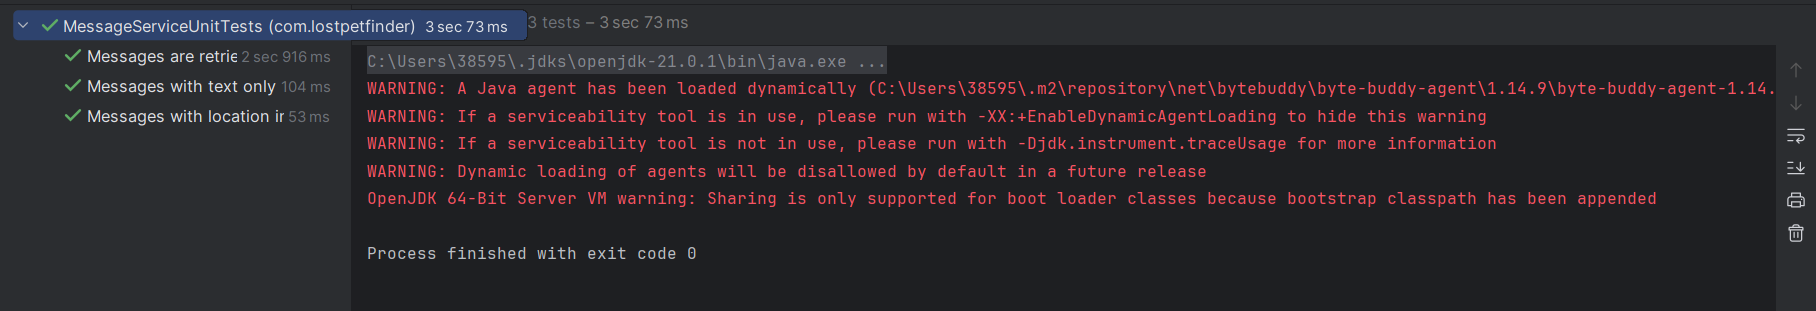
\includegraphics[width=\textwidth]{slike/test3.png}
	\caption{Testovi prolaze}
\end{figure}

\pagebreak

\subsection{Ispitivanje sustava}

Ispitivanje sustava proveli smo pomoću dodatka za preglednik
\underline{Selenium IDE} \footnote{https://www.selenium.dev/documentation/ide/}
te koristeći \underline{Selenium WebDriver}
\footnote{https://www.selenium.dev/documentation/webdriver/} unutar JUnit
testova.

\text{Ispitivanje pomoću Selenium WebDrivera prikazana su na slikama * i *}
\renewcommand{\lstlistingname}{Kod}
\begin{lstlisting}[
				language=Java,
				frame=single,
				label={lst:testLoginGoodCreds},
				basicstyle = \small,
				tabsize=2,
				showspaces=false,
				showstringspaces=false,
				commentstyle = \color{red}, %% set comment color
				keywordstyle = \color{blue}, %% set keyword color
				stringstyle = \color{applegreen}, %% set string color
				rulecolor = \color{black},
				caption={Test testLoginGoodCreds},
				breaklines=true]
@Test
public void testLoginGoodCreds() {
	WebDriver driver = new ChromeDriver();
	System.setProperty(
	"webdriver.chrome.driver", 
	"C:\\Users\\akrkl\\AppData\\Local\\Microsoft\\WindowsApps\\chromedriver.exe"
	);
	driver.manage().timeouts().implicitlyWait(10, TimeUnit.SECONDS);

	driver.get("http://localhost:5173/login");

	WebElement element = driver.findElement(By.id("email"));
	element.sendKeys("testadmin");

	element = driver.findElement(By.id("lozinka"));
	element.sendKeys("123");

	driver.findElement(By.cssSelector("button[type='submit']")).click();

	WebDriverWait wait = new WebDriverWait(driver, Duration.ofSeconds(2));
	try {
	wait.until(
		ExpectedConditions.presenceOfElementLocated(By.id("searchBarByCategories"))
	);

	String redirectUrl = driver.getCurrentUrl();

	Assertions.assertEquals(
		"http://localhost:5173/", redirectUrl
	);
	}
	finally {
	driver.quit();
	}
}	
			\end{lstlisting}

U Kodu \ref{lst:testLoginGoodCreds} testira se uspješan login korisnika. WebDriver otvara stranicu za login, pronalazi elemente za unos korisničkog imena i lozinke te unosi podatke. Nakon toga klikne na gumb za prijavu i čeka da se pojavi element za pretraživanje po kategorijama. Na kraju provjerava je li korisnik preusmjeren na početnu stranicu.

\pagebreak

\begin{lstlisting}[
				language=Java,
				frame=single,
				label={lst:testLoginBadCreds},
				basicstyle = \small,
				tabsize=2,
				showspaces=false,
				showstringspaces=false,
				commentstyle = \color{red}, %% set comment color
				keywordstyle = \color{blue}, %% set keyword color
				stringstyle = \color{applegreen}, %% set string color
				rulecolor = \color{black},
				caption={Test testLoginBadCreds},
				breaklines=true]
@Test
public void testLoginBadCreds() {
	WebDriver driver = new ChromeDriver();
	System.setProperty(
		"webdriver.chrome.driver",
		"C:\\Users\\akrkl\\AppData\\Local\\Microsoft\\WindowsApps\\chromedriver.exe"
	);
	driver.manage().timeouts().implicitlyWait(10, TimeUnit.SECONDS);
	driver.get("http://localhost:5173/login");

	WebElement element = driver.findElement(By.id("email"));
	element.sendKeys("testadmin");

	element = driver.findElement(By.id("lozinka"));
	element.sendKeys("wrongPassword");

	driver.findElement(By.cssSelector("button[type='submit']")).click();

	try {
		String redirectUrl = driver.getCurrentUrl();

		Assertions.assertNotEquals(
			"http://localhost:5173/", redirectUrl
		);
	}
	finally {
		driver.quit();
	}
}
			\end{lstlisting}

U Kodu \ref{lst:testLoginBadCreds} testira se neuspješan login korisnika. WebDriver otvara stranicu za login, pronalazi elemente za unos korisničkog imena i lozinke te unosi podatke. Nakon toga klikne na gumb za prijavu i provjerava je li korisnik preusmjeren na početnu stranicu.

\pagebreak

\begin{figure}[!htb]
	\centering
	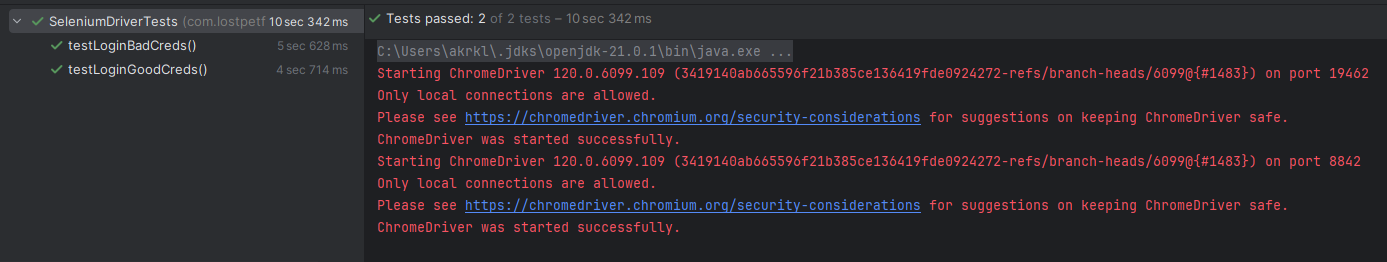
\includegraphics[width=\textwidth]{slike/test_passed.png}
	\caption{Testovi prolaze}
\end{figure}

\par\noindent\rule{\textwidth}{0.5pt}

\begin{figure}[!htb]
	\centering
	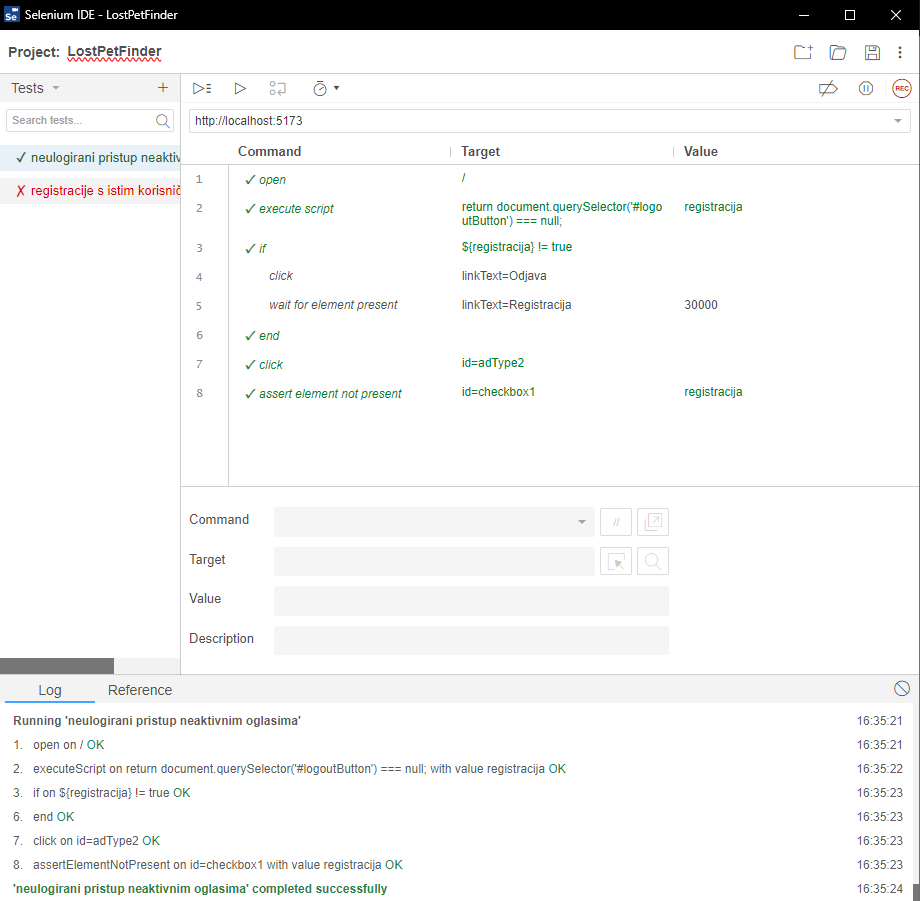
\includegraphics[width=\textwidth]{slike/selenium_test_1.png}
	\caption{Test: neulogirani korisnik pristupa neaktivnim oglasima}
\end{figure}

U ovom testu pomoću Selenium IDE-a provjerava se može li neulogirani korisnik pristupiti neaktivnim oglasima klikom na pripadajući radio button. Prvo se provjerava je li korisnik ulogiran, u tom slučaju se odjavljuje. Nakon toga se otvara stranica za prikaz oglasa, klikne se na radio button za prikaz neaktivnih oglasa i provjerava se je li se pojavio checkbox za filtriranje neaktivnih oglasa. Ako nije, test prolazi. Iz priloženog se vidi da aplikacija prolazi test.

\par\noindent\rule{\textwidth}{0.5pt}

\begin{figure}[!htb]
	\centering
	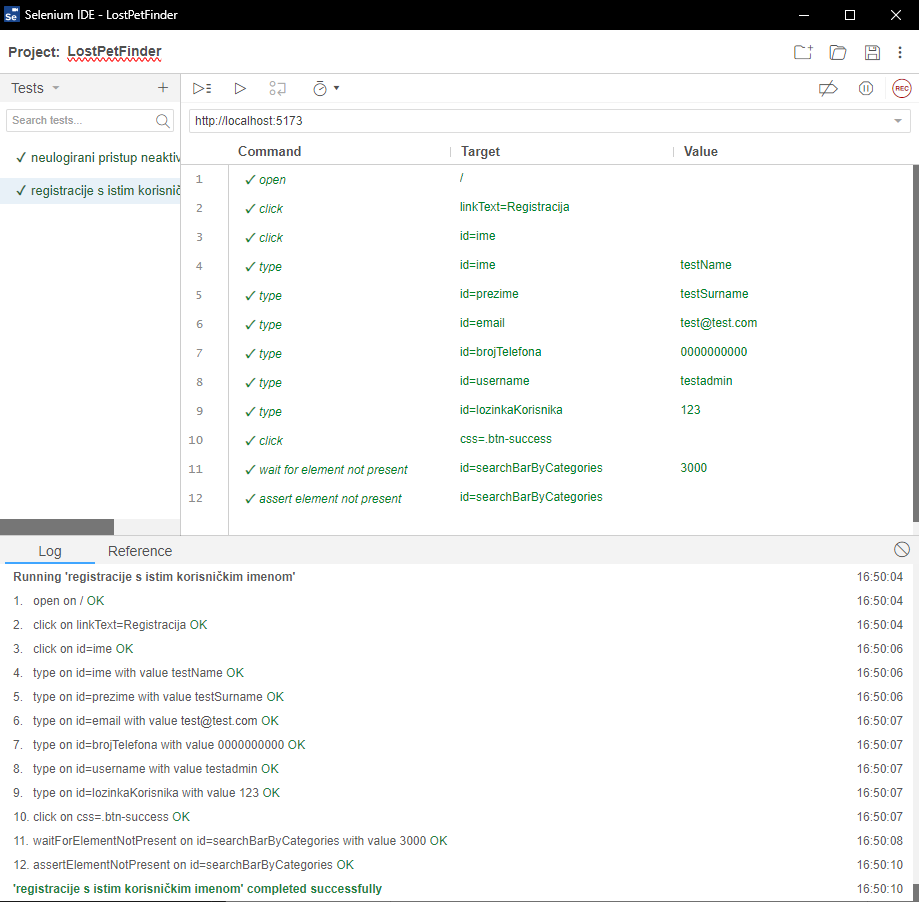
\includegraphics[width=\textwidth]{slike/selenium_test_2.png}
	\caption{Test: registracija s već postojećim podacima korisnika}
\end{figure}

U ovom testu pomoću Selenium IDE-a provjerava se kako aplikacija reagira na pokušaj registracije korisnika s podacima već postojećeg korisnika. Nakon unosa klikne se na gumb koji šalje formu i provjerava se je li se pojavio element za pretraživanje po kategorijama, odnosno je li se dogodio redirect na početnu stranicu. Ako nije, registracija nije uspjela i test prolazi. Iz priloženog se vidi da aplikacija prolazi test.

\eject


\section{Dijagram razmještaja}

\noindent Dijagrami razmještaja opisuju kako su komponente sustava raspoređene unutar njihovog radnog okruženja, uključujući sklopovlje i softversku podršku. Na poslužiteljskom računalu nalaze se web poslužitelj i poslužitelj baze podataka. Klijenti pristupaju web aplikaciji putem web preglednika. Arhitektura sustava temelji se na modelu "klijent-poslužitelj", gdje se komunikacija između računala korisnika (korisnik, registrirani korisnik, sklonište za životinje) i poslužitelja odvija preko HTTP veze.

\begin{figure}[!htb]
	\centering
	\includegraphics[width=\textwidth]{slike/Dijagram_razmještaja}
	\caption{Dijagram razmještaja}
\end{figure}

\eject

\section{Upute za puštanje u pogon}

\textit{Sljedeće upute prikazuju kako pustiti aplikaciju pogon pomoću servisa \underline{Render}\footnote{https://render.com/}.}

Izvorni kod aplikacije prvo treba pripremiti u svoj repozitorij na GitHubu (izradom forka repozitorija ove aplikacije) te bi trebalo izraditi korisnički račun na Renderu na koji treba povezati svoj GitHub račun. Nakon toga treba stvoriti novi poslužitelj na Renderu te u njega postaviti izvorni kod aplikacije. Za to je potrebno napraviti sljedeće korake:

\subsection{Izrada i postavljanje baze podataka aplikacije}

Proces izrade baze podataka je sljedeći:

\begin{enumerate}
	\item Na Render dashboardu odabrati \textit{New} -- \textit{PostgreSQL}.
	\item Popuniti polje \textit{Name} (proizvoljno).
	\item Odabrati \textit{PostgreSQL Version} -- 15.
	\item Odabrati tip stroja (za osnovnu funkcionalnost je dovoljan \textit{Free - 1 GB}).
	\item Odabrati \textit{Create Database}.
\end{enumerate}

Nakon što je baza podataka stvorena, potrebno je postaviti konfiguraciju backenda da se može povezati na nju. To se radi na sljedeći način:

\begin{enumerate}
	\item Na Render dashboardu odabrati bazu podataka nazvanu u prethodnom koraku.
	\item U kategoriji \textit{Info} pronaći skupinu \textit{Connections} u kojem se trebaju nalaziti sljedeća polja: \textit{Hostname}, \textit{Port}, \textit{Database}, \textit{Username}, \textit{Password} potrebna za idući korak.
	\item Na temelju tih podataka treba urediti/dodati segment u datoteci \textit{application.properties} koji se nalazi u direktoriju \textit{IzvorniKod/backend/src/main/resources} prema sljedećem obrascu:\\
	      \\
	      \verb+# Konfiguracija baze podataka+\\
	      \verb+spring.datasource.password=${DB_PASS:+\underline{\textlangle Password\textrangle}\verb+}+\\
	      \verb+spring.datasource.username=${DB_USERNAME:+\underline{\textlangle Username\textrangle}\verb+}+\\
	      \verb+spring.datasource.url=${DB_URL:jdbc:postgresql://+\underline{\textlangle Hostname\textrangle}\verb+:+\underline{\textlangle Port\textrangle}\verb+/+\underline{\textlangle Database\textrangle}\verb+}+
\end{enumerate}

\subsection{Puštanje u pogon backenda aplikacije}

Uz preduvjet da je baza podataka kreirana i konfigurirana ispravno, proces puštanja backenda u pogon je sljedeći:

\begin{enumerate}
	\item Na Render dashboardu odabrati \textit{New} -- \textit{Web Service}.
	\item Odabrati opciju \textit{Build and deploy from GitHub}.
	\item Odabrati repozitorij u kojem se nalazi izvorni kod aplikacije na povezanom GitHub računu pritiskom na tipku \textit{Connect} pokraj njega.
	\item Popuniti polje \textit{Name} s proizvoljnim imenom za backend.
	\item Odabrati odgovarajuću granu repozitorija u kojoj se nalazi izvorni kod aplikacije (obično je to \verb+main+).
	\item U polje \textit{Root Directory} upisati \verb+./IzvorniKod/backend+.
	\item Za \textit{Runtime} odabrati \textit{Docker}.
	\item Odabrati odgovarajući model računala u \textit{Instance Type}
	\item Na dnu stranice proširiti \textit{Advanced} opcije.
	\item U polje \textit{Dockerfile Path} upisati \verb+./Dockerfile+.
	\item Potvrditi izradu poslužitelja pritiskom na \textit{Create Web Service}.
	\item Nakon što se poslužitelj izradi, potrebno je kopirati adresu poslužitelja koja se nalazi ispod dodijeljenog imena poslužitelja nakon što se klikne na njega na Render dashboardu (adresa će biti potrebna pri konfiguraciji frontenda).
\end{enumerate}

\subsection{Puštanje u pogon frontenda aplikacije}

Nakon uspostavljanja backenda, sljedeći korak je puštanje u pogon frontenda. To se radi na sljedeći način:

\begin{enumerate}
	\item Na Render dashboardu odabrati \textit{New} -- \textit{Web Service}.
	\item Odabrati opciju \textit{Build and deploy from GitHub}.
	\item Odabrati repozitorij u kojem se nalazi izvorni kod aplikacije na povezanom GitHub računu pritiskom na tipku \textit{Connect} pokraj njega.
	\item Popuniti polje \textit{Name} s proizvoljnim imenom za frontend.
	\item Odabrati odgovarajuću granu repozitorija u kojoj se nalazi izvorni kod aplikacije (obično je to \verb+main+).
	\item U polje \textit{Root Directory} upisati \verb+./IzvorniKod/frontend+.
	\item Za \textit{Runtime} odabrati \textit{Node}.
	\item U polje \textit{Build Command} upisati \verb+yarn+.
	\item U polje \textit{Start Command} upisati \verb+yarn start-prod+.
	\item Odabrati odgovarajući model računala u \textit{Instance Type}.
	\item Potrebno je dodati dvije varijable okruženja u \textit{Environment Variables}:\\
	      \verb+API_BASE_URL+ s vrijednosti \verb+<Adresa poslužitelja backenda>+\\
	      \verb+PORT+ s vrijednosti \verb+5173+
\end{enumerate}

Nakon uspješnog postavljanja svih triju komponenti, aplikacija je spremna za korištenje te se može posjetiti na adresi koja je dodijeljena frontendu.


\eject
	\chapter{Zaključak i budući rad}

Zadatak naše grupe bio je razvoj web aplikacije za pronalazak nestalih ljubimaca gdje postoji mogućnost objavljivanja, izmjene i brisanja oglasa te razgovora putem chat-a s drugim sudionicima koji su uključeni u potragu za nestalim ljubimcima. Nakon 15 tjedana rada u timu i razvoja, ostvarili smo zadani cilj. Sama provedba projekta bila je kroz dvije faze.

Prva faza projekta uključivala je okupljanje tima za razvoj aplikacije, dodjelu projektnog zadatka i intenzivan rad na dokumentiranju zahtjeva. Kvaliteta provedbe prve faze uvelike je olakšala daljnji rad pri realizaciji osmišljenog sustava. Izrađeni obrasci i dijagrami(obrasci uporabe, sekvencijski dijagrami, model baze podataka, dijagram razreda) bili su od pomoći podtimovima zaduženima za razvoj \textit{backenda} i \textit{frontenda}. Izrada vizualnih prikaza idejnih rješenja problemskih zadataka uštedjela je mnogo vremena u drugom ciklusu kada su članovi tima nailazili na nedoumice oko implementacije rješenja.

Druga faza projekta, iako nešto kraća od prve, bila je puno intenzivnija po pitanju samostalnog rada članova. Manjak iskustva članova u izradi sličnih implementacijskih rješenja primorao je članove na samostalno učenje odabranih alata i programskih jezika kako bi ispunili dogovorene ciljeve. Osim realizacije rješenja, u drugoj fazi je bilo potrebno dokumentirati ostale UML dijagrame i izraditi popratnu dokumentaciju kako bi budući korisnici mogli lakše koristiti ili vršiti preinake na sustavu. Dobro izrađen kostur projekta uštedio nam je mnogo vremena prilikom izrade aplikacije te smo izbjegli moguće pogreške u izradi koje bi bile vremenski skupe za ispravljanje u daljnjoj fazi projekta.

Komunikacija među članovima tima bila je putem Discorda čime smo postigli informiranost svih članova grupe o napretku projekta. Moguće proširenje postojeće inačice sustava je izrada mobilne aplikacije čime bi cilj projektnog zadatka bio ostvaren u većoj mjeri.

Sudjelovanje na ovakvom projektu bio je vrijedno iskustvo svim članovima tima jer smo kroz intenzivnih nekoliko tjedana rada iskusili zajednički rad na istom projektu. Također, osjetili smo važnost dobre vremenske organiziranosti i koordiniranosti između članova tima. Zadovoljni smo postignutim bez obzira na golemi prostor za usavršavanje izrađene aplikacije što je posljedica neiskustva na takvim i sličnim projektima.

\eject
	\chapter*{Popis literature}
		\addcontentsline{toc}{chapter}{Popis literature}
	 	
 		\textbf{\textit{Kontinuirano osvježavanje}}
	
		\textit{Popisati sve reference i literaturu koja je pomogla pri ostvarivanju projekta.}
		
		
		\begin{enumerate}
			
			
			\item  Programsko inženjerstvo, FER ZEMRIS, \url{http://www.fer.hr/predmet/proinz}
			
			\item  I. Sommerville, "Software engineering", 8th ed, Addison Wesley, 2007.
			
			\item  T.C.Lethbridge, R.Langaniere, "Object-Oriented Software Engineering", 2nd ed. McGraw-Hill, 2005.
			
			\item  I. Marsic, Software engineering book``, Department of Electrical and Computer Engineering, Rutgers University, \url{http://www.ece.rutgers.edu/~marsic/books/SE}
			
			\item  The Unified Modeling Language, \url{https://www.uml-diagrams.org/}
			
			\item  Astah Community, \url{http://astah.net/editions/uml-new}
		\end{enumerate}
		
		 
	
	
	\begingroup
	\renewcommand*\listfigurename{Indeks slika i dijagrama}
	%\renewcommand*\listtablename{Indeks tablica}
	%\let\clearpage\relax
	\listoffigures
	%\vspace{10mm}
	%\listoftables
	\endgroup
	\addcontentsline{toc}{chapter}{Indeks slika i dijagrama}


	
	\eject 
		
	\chapter*{Dodatak: Prikaz aktivnosti grupe}
\addcontentsline{toc}{chapter}{Dodatak: Prikaz aktivnosti grupe}

\section*{Dnevnik sastajanja}

\begin{packed_enum}
	\item  sastanak

	\item[] \begin{packed_item}
		\item Datum: 16. listopada 2023.
		\item Prisustvovali: A. Krklec, P. Marinić, V. Mesar, A. Prskalo, L. Raić, L. Rogoz, R. Vitaliani
		\item Teme sastanka:
		\begin{packed_item}
			\item sastanak s asistentom i demonstratorom
			\item raščišćavanje osnovnih dilema funkcionalnosti
			\item analiza zadatka
			\item plan i razrada obrade projektnog zadatka
			\item definiranje i dodjela poslova
		\end{packed_item}
	\end{packed_item}

	\item  sastanak
	\item[] \begin{packed_item}
		\item Datum: 28. listopada 2023.
		\item Prisustvovali: A. Krklec, P. Marinić, V. Mesar, A. Prskalo, L. Raić, L. Rogoz, R. Vitaliani
		\item Teme sastanka:
		\begin{packed_item}
			\item konačan odabir alata i tehnologija
			\item podjela rada
			\item opis projektnog zadatka
			\item funkcionalni zahtjevi, aktori i dionici
			\item ostali zahtjevi
			\item dijagrami obrazaca uporabe
			\item opis obrazaca uporabe
		\end{packed_item}
	\end{packed_item}

	\item  sastanak
	\item[] \begin{packed_item}
		\item Datum: 5. studenog 2023.
		\item Prisustvovali: A. Krklec, P. Marinić, V. Mesar, A. Prskalo, L. Raić, L. Rogoz, R. Vitaliani
		\item Teme sastanka:
		\begin{packed_item}
			\item daljnja podjela rada
			\item sekvencijski dijagrami
			\item dijagram baze podataka
			\item opis arhitekture i dizajn sustava
			\item osmišljavanje stranice i pojedinih pregleda
			\item početak rada na backendu i frontendu
		\end{packed_item}
	\end{packed_item}

	\item  sastanak
	\item[] \begin{packed_item}
		\item Datum: 10. studenog 2023.
		\item Prisustvovali: A. Krklec, P. Marinić, V. Mesar, A. Prskalo, L. Raić, L. Rogoz, R. Vitaliani
		\item Teme sastanka:
		\begin{packed_item}
			\item daljnja podjela rada
			\item opis baze podataka
			\item opis tablica baze podataka
			\item opis arhitekture i dizajn sustava
			\item rad na backendu i frontendu
		\end{packed_item}
	\end{packed_item}

	\item  sastanak
	\item[] \begin{packed_item}
		\item Datum: 13. studenog 2023.
		\item Prisustvovali: A. Krklec, P. Marinić, V. Mesar, A. Prskalo, L. Raić, L. Rogoz, R. Vitaliani
		\item Teme sastanka:
		\begin{packed_item}
			\item prva revizija dijagrama razreda
			\item opis dijagrama razreda
			\item sastanak s asistentom i demonstratorom - evaluacija rada
		\end{packed_item}
	\end{packed_item}

	\item  sastanak
	\item[] \begin{packed_item}
		\item Datum: 16. studenog 2023.
		\item Prisustvovali: A. Krklec, P. Marinić, V. Mesar, A. Prskalo, L. Raić, L. Rogoz, R. Vitaliani
		\item Teme sastanka:
		\begin{packed_item}
			\item privođenje 1. revizije web aplikacije i dokumentacije kraju
			\item aplikacija puštena u pogon i poslane informacije o korisničkim imenima
		\end{packed_item}
	\end{packed_item}

	\item  sastanak
	\item[] \begin{packed_item}
		\item Datum: 17. prosinca 2023.
		\item Prisustvovali: A. Krklec, P. Marinić, V. Mesar, A. Prskalo, L. Raić, L. Rogoz, R. Vitaliani
		\item Teme sastanka:
		\begin{packed_item}
			\item opis dijagrama stanja
			\item opis dijagrama aktivnosti
			\item planiranje rada na frontendu i backendu
		\end{packed_item}
	\end{packed_item}

	\item  sastanak
	\item[] \begin{packed_item}
		\item Datum: 18. prosinca 2023.
		\item Prisustvovali: A. Krklec, P. Marinić, V. Mesar, A. Prskalo, L. Raić, L. Rogoz, R. Vitaliani
		\item Teme sastanka:
		\begin{packed_item}
			\item rad na frontendu i backendu
			\item planiranje daljnjih poslova
		\end{packed_item}
	\end{packed_item}

	\item  sastanak
	\item[] \begin{packed_item}
		\item Datum: 21. prosinca 2023.
		\item Prisustvovali: A. Krklec, P. Marinić, V. Mesar, A. Prskalo, L. Raić, L. Rogoz, R. Vitaliani
		\item Teme sastanka:
		\begin{packed_item}
			\item opis dijagrama komponenti
			\item opis dijagrama razmještaja
			\item rad na frontendu i backendu
		\end{packed_item}
	\end{packed_item}

	\item  sastanak
	\item[] \begin{packed_item}
		\item Datum: 14. siječnja 2024.
		\item Prisustvovali: A. Krklec, P. Marinić, V. Mesar, A. Prskalo, L. Raić, L. Rogoz, R. Vitaliani
		\item Teme sastanka:
		\begin{packed_item}
			\item ažurirani dijagrami razreda
			\item ispravak sekvencijskih dijagrama
			\item mala izmjena opisa projektnog zadatka
		\end{packed_item}
	\end{packed_item}
	
	\item  sastanak
	\item[] \begin{packed_item}
		\item Datum: 17. siječnja 2024.
		\item Prisustvovali: A. Krklec, P. Marinić, V. Mesar, A. Prskalo, L. Raić, L. Rogoz, R. Vitaliani
		\item Teme sastanka:
		\begin{packed_item}
			\item dodane korištene tehnologije i alati
			\item dodan zaključak i budući rad
		\end{packed_item}
	\end{packed_item}
	
	\item  sastanak
	\item[] \begin{packed_item}
		\item Datum: 17. siječnja 2024.
		\item Prisustvovali: A. Krklec, P. Marinić, V. Mesar, A. Prskalo, L. Raić, L. Rogoz, R. Vitaliani
		\item Teme sastanka:
		\begin{packed_item}
			\item dodane upute za puštanje u pogon
			\item dodana prezentacija
			\item popravljen dijagram obrazaca uporabe
			\item dodana dokumentacija za ispitivanje komponenti sustava
			\item ažurirani dijagrami razreda
			\item završetak implementacije
			\item dovršavanje pisanja dokumentacije
		\end{packed_item}
	\end{packed_item}

	%

\end{packed_enum}

\eject
\section*{Tablica aktivnosti}

\begin{longtblr}[
	label=none,
	]{
	vlines,hlines,
	width = \textwidth,
	colspec={X[7, l]X[1, c]X[1, c]X[1, c]X[1, c]X[1, c]X[1, c]X[1, c]},
	vline{1} = {1}{text=\clap{}},
	hline{1} = {1}{text=\clap{}},
	rowhead = 1,
	}

	\SetCell[c=1]{c}{}                               & \SetCell[c=1]{c}{\rotatebox{90}{\textbf{Patrik Marinić}}} & \SetCell[c=1]{c}{\rotatebox{90}{\textbf{Andrija Krklec }}} & \SetCell[c=1]{c}{\rotatebox{90}{\textbf{Vedran Mesar }}} & \SetCell[c=1]{c}{\rotatebox{90}{\textbf{Anđelko Prskalo }}} & \SetCell[c=1]{c}{\rotatebox{90}{\textbf{Luka Raić }}} & \SetCell[c=1]{c}{\rotatebox{90}{\textbf{Luka Rogoz }}} & \SetCell[c=1]{c}{\rotatebox{90}{\textbf{Robert Vitaliani }}} \\
	Upravljanje projektom                            & 8                                                         &                                                            &                                                          &                                                             &                                                       &                                                        &                                                              \\
	Opis projektnog zadatka                          & 3                                                         &                                                            &                                                          &                                                             &                                                       &                                                        & 5                                                            \\

	Funkcionalni zahtjevi                            &                                                           &                                                            &                                                          &                                                             & 3                                                     & 5                                                      &                                                              \\
	Opis pojedinih obrazaca                          &                                                           & 6                                                          &                                                          &                                                             & 2                                                     &                                                        &                                                              \\
	Dijagram obrazaca                                &                                                           &                                                            &                                                          &                                                             & 5                                                     &                                                        &                                                              \\
	Sekvencijski dijagrami                           &                                                           &                                                            &                                                          & 7                                                           &                                                       &                                                        &                                                              \\
	Opis ostalih zahtjeva                            &                                                           & 2                                                          &                                                          &                                                             &                                                       &                                                        &                                                              \\

	Arhitektura i dizajn sustava                     &                                                           & 3                                                          &                                                          &                                                             &                                                       &                                                        &                                                              \\
	Baza podataka                                    &                                                           &                                                            &                                                          &                                                             &                                                       & 6                                                      &                                                              \\
	Dijagram razreda                                 &                                                           &                                                            & 6                                                        &                                                             & 3                                                     & 5                                                      &                                                              \\
	Dijagram stanja                                  &                                                           &                                                            &                                                          &                                                             &                                                       & 5                                                      &                                                              \\
	Dijagram aktivnosti                              &                                                           &                                                            & 2                                                        &                                                             &                                                       & 4                                                      &                                                              \\
	Dijagram komponenti                              &                                                           &                                                            & 5                                                        &                                                             &                                                       &                                                        &                                                              \\
	Korištene tehnologije i alati                    & 1                                                         &                                                            &                                                          & 1                                                           &                                                       &                                                        & 3                                                            \\
	Ispitivanje programskog rješenja                 & 4                                                         & 12                                                         & 3                                                        & 5                                                           & 13                                                    & 2                                                      & 9                                                            \\
	Dijagram razmještaja                             &                                                           &                                                            & 4                                                        &                                                             &                                                       & 2                                                      &                                                              \\
	Upute za puštanje u pogon                        &                                                           & 6                                                          &                                                          & 11                                                          &                                                       &                                                        & 3                                                            \\
	Dnevnik sastajanja                               & 2                                                         &                                                            &                                                          &                                                             &                                                       &                                                        & 4                                                            \\
	Zaključak i budući rad                           &                                                           &                                                            &                                                          &                                                             &                                                       &                                                        & 3                                                            \\
	Popis literature                                 & 2                                                         & 2                                                          & 2                                                        & 2                                                           & 2                                                     & 2                                                      & 2                                                            \\ \hline
	\textit{Izrada baze podataka}                    &                                                           & 5                                                          &                                                          &                                                             & 6                                                     & 8                                                      &                                                              \\
	\textit{Spajanje s bazom podataka}               & 1                                                         & 4                                                          & 1                                                        & 3                                                           & 4                                                     & 2                                                      & 1                                                            \\
	\textit{Korisnička autentikacija i autorizacija} & 1                                                         & 5                                                          &                                                          &                                                             & 5                                                     & 1                                                      & 2                                                            \\
	\textit{Backend}                                 &                                                           & 60                                                         & 14                                                       & 10                                                          & 50                                                    & 6                                                      &                                                              \\
	\textit{Frontend}                                & 45                                                        &                                                            &                                                          &                                                             &                                                       &                                                        & 60                                                           \\
	\textit{Testiranje}                              & 7                                                         & 8                                                          & 4                                                        & 4                                                           & 8                                                     & 4                                                      & 9                                                            \\
	\textit{Deploy}                                  &                                                           & 6                                                          &                                                          & 16                                                          &                                                       &                                                        &                                                              \\
\end{longtblr}


\eject
\section*{Dijagrami pregleda promjena}

\begin{figure}[H]
	\centering
	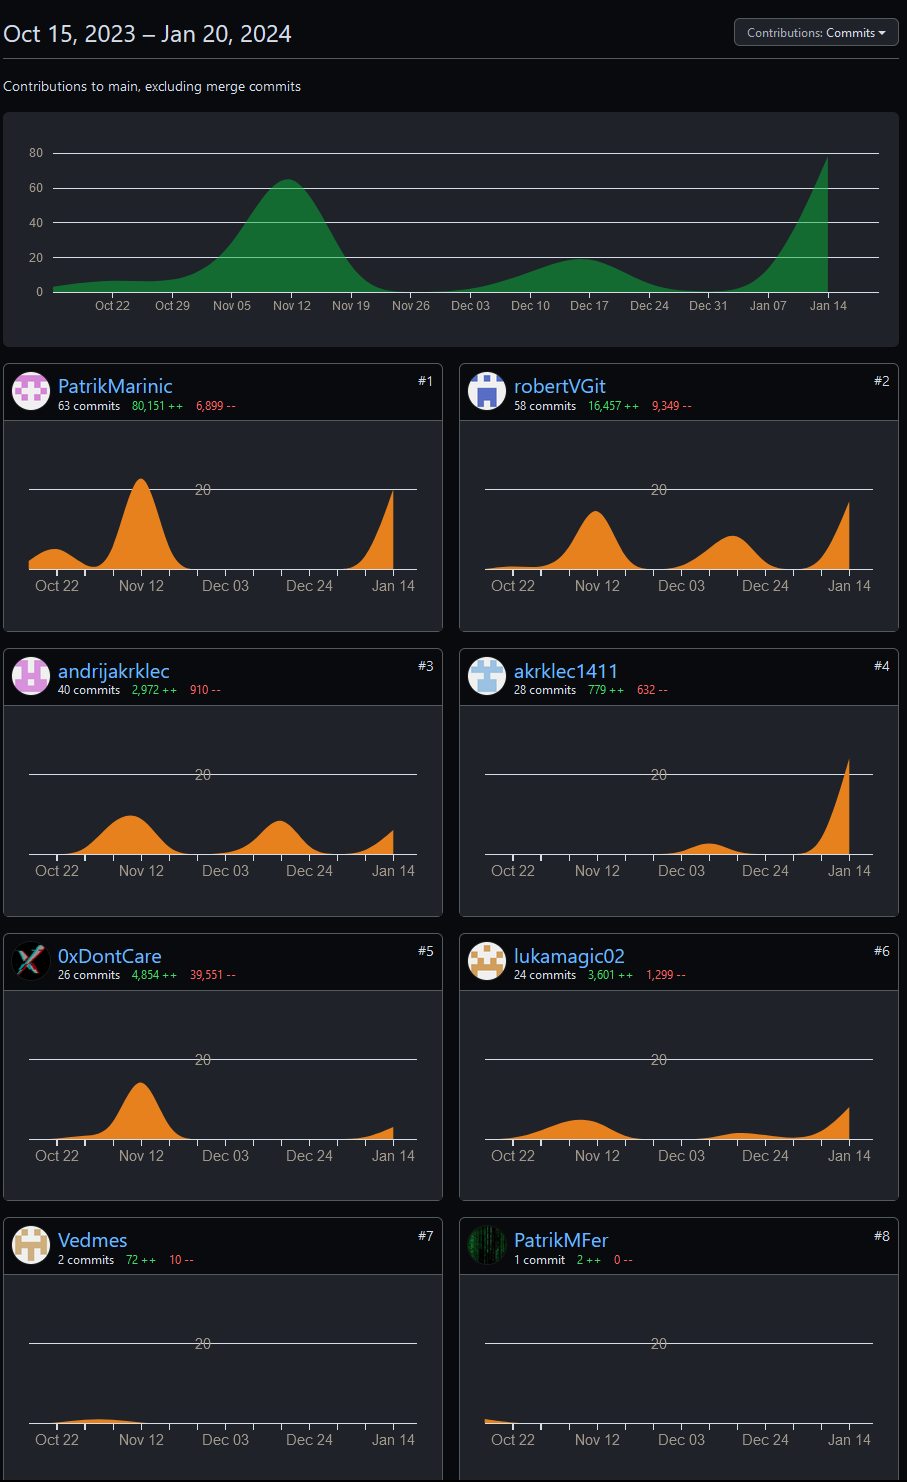
\includegraphics[scale=0.5]{slike/aktivnost.PNG}
	\caption{Prikaz aktivnosti na repozitoriju}
	\label{fig:promjene1}
\end{figure}




\end{document} %naredbe i tekst nakon ove naredbe ne ulaze u izgrađen dokument 


